\chapter{Clusterify}
	Clusterify è un'applicazione web che offre agli utenti la possibilità di leggere gli stessi tweet che leggerebbero sul loro \emph{newsfeed}, organizzati, però, in insiemi definiti dinamicamente in modo da permettere loro di soffermarsi solamente su testi appartenenti a categorie che questi reputano interessanti. L'idea di quest'applicazione è nata dal bisogno di non voler leggere tutti i tweet che una determinata persona pubblica. 

	Supponiamo che un utente $X$, aspirante cuoco, segua $Y$, cuoca neo-mamma conosciuta a livello nazionale. Quest'ultima pubblica due tweet:
	\begin{inparaenum}[\itshape 1\upshape)]
		\item \#Plumcake alla \#Nutella: continuano gli esperimenti @GialloZafferano ;)
		\item Giocare una battaglia a \#palledineve e perdere con il proprio piccolo di 3 anni <3
	\end{inparaenum}.
	Probabilmente $X$ sarà molto interessato alla ricetta del \emph{Plumcake} ma, al contempo, non attratto dalla vita personale di $Y$.

	Clusterify dividerà questi tweet in gruppi distinti ed $X$ avrà la possibilità di leggere solo quelli riferiti ad ambiti culinari senza essere disturbato da storie di vita personale, recensioni di film e quant'altro.

\section{Background}
	Clusterify nasce con lo scopo di raggruppare per argomenti i tweet presenti nel newsfeed di un qualsiasi utente. Per questo scopo è necessario attribuire ad ogni tweet gli argomenti di cui tratta raggruppandoli per quanto questi siano collegati tra di loro. 

	Si è deciso di utilizzare la \emph{Twitter API} per ottenere dati da twitter e \emph{dataTXT} per estrarre gli argomenti e calcolarne le varie relazioni.

	\subsection{Twitter API}
	Twitter Inc. è un social network che permette ai propri utenti di scrivere e di leggere \emph{micropost}, messaggi lunghi al più 140 caratteri, comunemente chiamati \emph{tweet}. 

	Questa piattaforma, creata nel 2006 da Jack Dorsey, Evan Williams, Biz Stone e Noah Glass, ha spopolato fino a raggiungere nel 2013 più di 200 milioni di utenti attivi e più di 400 milioni di visite al giorno\cite{twitter_data}.

	Ad oggi, Twitter è l'undicesimo sito internet visitato quotidianamente, secondo nei social network, preceduto solamente da Facebook\cite{twitter_alexa}.

	Twitter possiede, come la maggior parte dei social network, un servizio interrogabile via API per ottenere e per caricare dati: nel primo caso si possono richiedere i tweet che compongono il \emph{newsfeed} di un dato utente, i messaggi privati che due utenti si scambiano ed ancora alcuni dati relativi al profilo, come nome e cognome, nickname, immagine utente e così via; nel secondo caso, invece, si può pubblicare un tweet come se l'utente lo facesse dall'interfaccia web oppure modificare dati che Twitter ha salvato nel proprio database. 

	In entrambi i casi serve che l'utente interessato ``firmi'' un consenso che permetterà al programmatore di interagire con questi dati. 

	\subsubsection{REST API v1.1}
		Il modo che Twitter offre per interagire con i propri dati è la REST API. 
	
		Con REST (Representational State Transfer) si indica un tipo di architettura software basato sull'idea di utilizzare la comunicazione tra macchine per mezzo di richieste HTTP.

		Le applicazioni basate su questo tipo di architettura vengono chiamate RESTful ed utilizzano, appunto, HTTP per tutte le operazioni di \emph{CRUD}: Create, Read, Update e Remove.

		Twitter mette a disposizione, nella documentazione per i programmatori\cite{twitter_doc}, una lunga lista di possibili richieste -- \url{https://dev.twitter.com/docs/api/1.1} -- e, per ognuna di queste, una pagina dedicata dove vengono elencati i dati richiesti in input, i possibili filtri applicabili, la struttura dell'output che questa richiesta genererà ed infine un esempio richiesta/risposta per chiarire le idee.

		% https://dev.twitter.com/docs/auth
		OAuth, il protocollo di autenticazione che Twitter utilizza\cite{twitter_auth}, permette agli utenti di approvare che un'applicazione agisca al loro posto, senza il bisogno di condividere i dati sensibili, quali username e password. OAuth scambia dei token per evitare il passaggio di questa tipologia di dati.

		Gli sviluppatori possono così pubblicare e interagire con dati protetti, come ad esempio i service provider e al contempo proteggono le credenziali dei loro utenti\cite{twitter_auth_faq}.

% PARLARE DI UNA POSSIBILE RICHIESTA!
	\subsection{dataTXT}
% https://www.mashape.com/dandelion/datatxt-1#!documentation
	DataTXT è un insieme di API semantiche sviluppate da SpazioDati S.r.l.  -- \url{http://spaziodati.eu} -- che mira a estrarre significato da testi scritti in diverse lingue. Questo prodotto si diversifica dagli altri dello stesso genere in quanto è stato pensato e ottimizzato per lavorare su testi molto corti, come i tweet.

	DataTXT può estrarre da un testo delle \emph{entità}, può categorizzare documenti in categorie stabilite dall'utente stesso e molto altro.

	%\subsubsection{Grafo di dataTXT}
%		DataTXT per poter eseguire i suoi algoritmi ha bisogno di basarsi su di un grafo pre-calcolato; questo ha $n+r$ nodi, dove $n$ sono gli snippet $S =  \{S_1, ..., S_n\}$ e $r$ sono i topic $T = \{t_1, ..., t_r\}$. 
%
%		Dato uno snippet $s$ e un topic $t$, denotiamo come $p(s,t)$ lo score che dataTXT assegna all'annotazione di $s$ con il topic $t$. Questo valore rappresenta l'importanza che un topic $t$ ha su di uno snippet $s$ e viene utilizzato come valore per l'arco da va da $s$ a $t$ nel grafo stesso.
%
%	Dati due topic $t_a$ e $t_b$, per esempio due pagine di Wikipedia, si può misurare la loro \emph{relatedness} $rel(t_a, t_b)$ utilizzano la seguente funzione che si basta sul numero di citazioni e co-citazioni delle due pagine di Wikipedia:
%	\begin{equation*}
%	  rel(t_a, t_b) = \frac{log(| in(t_a) |) - log(| in(t_a) \cap in(t_b)|)}{log(W) - log(|in(t_b)|)}
%	\end{equation*}
%	dove $in(t)$ è il set di archi entranti nella pagina $t$ e $W$ è il numero totale delle pagine di Wikipedia\cite{datatxt_graph}.

	\subsubsection{dataTXT NEX}
		DataTXT NEX (\emph{Named Entity eXtraction}) è un API che permette di localizzare e di estrarre da un testo entità quali persone, organizzazioni, luoghi, espressioni di tempo, ecc.

		Per ottenere queste informazioni basta richiedere via HTTP l'elaborazione dei dati  prefissati in input. Segue un esempio: \url{https://api.dandelion.eu/datatxt/nex/v1/?lang=en&text=The%20doctor%20says%20an%20apple%20is%20better%20than%20an%20orange&include=type,abstract,categories,lod&$app_id=YOUR_APP_ID&$app_key=YOUR_APP_KEY}

		Dopo l'elaborazione di una qualsiasi richiesta, una risposta viene consegnata.

		Come  tutte le chiamate HTTP, anche le risposte di dataTXT sono composte da un \emph{header} e da un \emph{body}.

		Nella prima sezione sono presenti molte informazioni utili quali il numero di crediti utilizzati, quelli rimanenti e la data in cui questi torneranno al valore iniziale, come di seguito mostrato:
		
		\begin{lstlisting}
Connection: keep-alive
Content-Length: 2748
Content-Type: application/json;charset=UTF-8
Date: Wed, 21 Oct 2015 16:29:37 GMT
Server: Apache-Coyote/1.1
X-DL-units: 1
X-DL-units-left: 999
X-DL-units-reset: 2015-10-22 00:00:00 +0000
		\end{lstlisting}

		Nella seconda, invece, sono presenti i dati veri e propri. \emph{Annotations} è la lista composta dagli elementi trovati, con vari dettagli; questi elementi sono filtrati da alcuni parametri che possono essere passati nella richiesta,  ad esempio la \emph{min\_confidence}.

		\begin{lstlisting}
{
  "timestamp": "2015-10-21T16:29:37",
  "time": 2,
  "lang": "en",
  "annotations": [{
      "...": "...",
  }, {
    "abstract": "The apple is the fruit of the apple tree...",
    "id": 18978754,
    "title": "Apple",
    "start": 19,
    "categories": [
      "Apples",
      "Malus",
      "Plants described in 1803",
      "Sequenced genomes"
    ],
    "lod": {
      "wikipedia": "http://en.wikipedia.org/wiki/Apple",
      "dbpedia": "http://dbpedia.org/resource/Apple"
    },
    "label": "Apple",
    "types": [
      "http://dbpedia.org/ontology/Eukaryote",
      "http://dbpedia.org/ontology/Plant",
      "http://dbpedia.org/ontology/Species"
    ],
    "confidence": 0.7869,
    "uri": "http://en.wikipedia.org/wiki/Apple",
    "end": 24,
    "spot": "apple"
  }, {
    "...": "...",
  }]
}
		\end{lstlisting}

	\subsubsection{dataTXT REL}
		DataTXT REL  è un servizio che, ad oggi, non è ancora presente sul mercato ma che permetterà di capire quando un topic $t_a$ è correlato ad un topic $t_b$, ricavando questo valore dalla seguente formula:
		\begin{equation*}
			rel(t_a, t_b) = \frac{log(| in(t_a) |) - log(| in(t_a) \cap in(t_b)|)}{log(W) - log(|in(t_b)|)}
		\end{equation*}
		dove $in(t)$ è il set di archi entranti nella pagina $t$ e $W$ è il numero totale delle pagine di Wikipedia\cite{datatxt_graph}.

		Come dataTXT-NEX, anche dataTXT-REL sarà interrogabile nello stesso modo: \url{https://api.dandelion.eu/datatxt/rel/v1/?topic1=Roma&topic2=Trento&lang=it&$app_id=YOUR_APP_ID&$app_key=YOUR_APP_KEY}.

		L'\emph{header} della risposta sarà uguale a quello di dataTXT-NEX, mentre il \emph{body} sarà strutturato come segue:

		\begin{lstlisting}
{
  "time": 2,
  "relatedness": [{
    "weight": 0.7127059,
      "topic1": {
        "input": "Roma",
        "topic": {
          "id": 1209297,
          'title": "Roma",
          "uri": "http://it.wikipedia.org/wiki/Roma",
          "labe"l: "Roma"
        }
      },
      "topic2": {
        "input": "Trento",
        "topic": {
          "id": 100137,
          "title": "Trento",
          "uri": "http://it.wikipedia.org/wiki/Trento",
          "label": "Trento"
        }
      }
  }],
  "lang": "it",
  "timestamp": "2014-05-14T21:41:58.171"
}
		\end{lstlisting}




\section{Backend}
	Clusterify è un'applicazione Django -- \url{https://www.djangoproject.com/} -- pensata e creata basandosi sulla necessità di essere estesa e modellata secondo le preferenze degli sviluppatori. %inserire nuovi \emph{reader} e nuovi algoritmi di clustering. 

	Si può vedere il tutto come una struttura a mattoncini dove si possono scambiare dei blocchi per raggiungere il risultato atteso, senza necessariamente modificare il codice del \emph{core}. Questi blocchi sono i \emph{reader}, i \emph{livelli d cache} e gli \emph{algoritmi di cluster}.
	
	Permettere di ottenere testi da più fonti significa creare altrettanti mezzi per interfacciare Clusterify a queste sorgenti, creando una \emph{black-box} che trasforma i testi in input in un dato strutturato precedentemente definito. Clusterify nasce con TwitterReader che, come da nome, permette di leggere i dati direttamente dalle API di Twitter. Per creare un nuovo reader, quindi, basta soddisfare queste due regole.

	La cache, invece, è una componente strutturale che viene utilizzata da tutto il progetto per evitare il replicarsi di richieste HTTP già fatte. Clusterify nasce con Redis -- \url{http://redis.io/} -- integrato, permettendo comunque di cambiare questa componente se lo sviluppatore lo desidera.

	L'ultima componente estendibile sono gli algoritmi di clustering.

	\subsection{Algoritmi di clustering}
		Un algoritmo di clustering permette di raggruppare oggetti all'interno di insiemi, mantenendo uniti gli elementi che secondo alcune regole risultano più coesi e dividendo quelli meno simili.

		Poiché non esiste un algoritmo ottimo per ogni caso pensabile, Clusterify ne comprende \emph{quattro} nel core. Questi sono utili sia a rilasciare un sistema in grado di coprire la maggior parte dei casi d'uso, sia per valutare qual'è la performance migliore con l'input in questione.

		I quattro algoritmi presenti in Clusterify sono presi da scikit-learn -- \url{http://scikit-learn.org/}. Questa decisione è stata presa sia per offrire più di un algoritmo alla community, sia per valutare se la mia ipotesi iniziale circa il miglior algoritmo fosse corretta. 

		Questi algoritmi sono \emph{K-means}, \emph{Spectral}, \emph{Affinity Propagation} e \emph{Ward}.

		\subsubsection{K-means}
			K-means è il nome di un algoritmo di clustering che punta a creare $k$  gruppi distinti di uguale varianza, minimizzando l'inerzia del gruppo. Questo algoritmo richiede che il numero di cluster sia definito a priori. 

L'algoritmo punta a scegliere $k$ centroidi $C$ che minimizzano lo scarto quadratico medio con un dataset $X$ di $n$ elementi $(x_1,..., x_n)$, creando $k$ insiemi $S = {S_1, ..., S_K}$:

\begin{equation*}
	\underset {\mathbf{S}} {\operatorname{arg\,min}}  \sum_{i=1}^{k} \sum_{\mathbf x_j \in S_i} || x_j - \mu_i ||^2 
\end{equation*}

L'algoritmo in se è composto da tre passi:
\begin{enumerate}
	\item Scelta dei centroidi iniziali;
	\item Assegnamento di ogni componente;
	\item Creazione di nuovi centroidi;
\end{enumerate}

Dopo aver scelto i primi $k$ centroidi dalle componenti del dataset $X$, l'algoritmo continua ad eseguire due operazioni finché i centroidi proposti possono essere considerati corretti, ovvero che la propria posizione non venga modificata con il passare delle iterazioni. 

L'assegnamento di ogni componente ad un centroide si esegue utilizzando la distanza euclidea al quadrato, questa sarà assegnata al punto medio più vicino; si può calcolare la distribuzione delle componenti in questo modo:
\begin{equation*}
	S_i^{(t)} = \big \{ x_p : || x_p - m^{(t)}_i ||^2 \le || x_p - m^{(t)}_j ||^2 \ \forall j, 1 \le j \le k \big\}
\end{equation*}
dove ogni $x_p$ è assegnato a esattamente un $S^{(t)}$, anche se idealmente potrebbe essere assegnato a più di un centroide.

La creazione dei nuovi centroidi utilizza, invece, il valore medio di ogni componente appartenente ad ogni centroide precedentemente definito.
\begin{equation*}
	m^{(t+1)}_i = \frac{1}{|S^{(t)}_i|} \sum_{x_j \in S^{(t)}_i} x_j 
\end{equation*}

Per quanto riguarda la scelta dei centroidi ci si può basare sul caso, scegliendo in modo \emph{random} i punti, con l'idea che con il passare delle iterazioni queste stime si sistemeranno; la seconda scelta vede il posizionamento dei centroidi in modo equidistante dagli tra loro, col fine di cercare di massimizzare l'area coperta e minimizzare il numero di iterazioni necessarie per giungere nella situazione finale di stallo.

		\subsubsection{Spectral}
			Spectral è il nome di un algoritmo di clustering che punta ad utilizzare gli autovalori della matrice delle adiacenze per capire come partizionare gli elementi dell'insieme.

Dato un grafo, rappresentato appunto dalla matrice delle adiacenze, l'algoritmo cerca il taglio minimo all'interno del grafo ed elimina gli archi che passano dal primo insieme al secondo. Questo procedimento continua in modo iterativo finche non si raggiungono, come nel caso del k-means $k$ cluster.s

Lo spectral basa il suo funzionamento sulla matrice $A$ della adiacenze, simmetrica per definizione, con $A_{ij}\geq 0$ rappresentante la similarità tra l'elemento in indice $i$ e quello in indice $j$; questa matrice, conosciuta con il nome di matrice normalizzata di Laplace, viene definita in questo modo:

\begin{equation*}
	L^{norm} = I-D^{-1/2} A D^{-1/2},
\end{equation*}
dove $D$ è la matrice diagonale costruita in questo modo:
\begin{equation*}
	D_{ii} = \sum_j A_{ij}.
\end{equation*}

L'algoritmo partiziona gli elementi in due insiemi distinti ($B_1$, $B_2$) basando la scelta del taglio sui valori dell'autovettore $v$ relativo al secondo più piccolo autovalore calcolato su $L^{norm}.

		\subsubsection{Affinity Propagation}
			Affinity Propagation è un algoritmo di clustering basato sul concetto di "passaggio di messaggi" tra le varie componenti. Una caratteristica fondamentale di quest'algoritmo è la mancanza di necessità di determinare a priori la quantità di cluster che saranno necessari.

Un dataset è descritto utilizzando degli esemplari identificati come le componenti più rappresentative dell'insieme. I messaggi trasmessi tra coppie sono utilizzati per calcolare l'idoneità che una componente ha di essere l'esemplare dell'altra. Quest'ultima sarà successivamente aggiornata con i valori provenienti dalle altre coppie. Questo processo viene ripetuto iterativamente finché il tutto non converge, dando vita al cluster.

Sia $(x_1, ..., x_n)$ l'insieme dei punti da clusterizzare e sia $S$ una funzione che permette di definire la similarità di due punti.

L'algoritmo procede alternando due fasi di "passaggio di messaggi", aggiornando due matrici:

\begin{itemize}
	\item La matrice di responsabilità $R$ ha valori $r(i, k)$ che quantificano quanto $x_k$ sia ben situato nel cluster contenente $x_i$, prendendo in considerazione tutti gli altri elementi contenuti in questo insieme;
	\item La matrice di disponibilità $A$ contiene i valori $a(i, k)$ che rappresentano quanto sia appropriato per $x_i$ scegliere $x_k$ come prossimo elemento del cluster a cui lui stesso appartiene.
\end{itemize} 

Entrambe queste matrici sono inizializzate a $0$ e, successivamente, saranno aggiornate in modo iterativo con le seguenti espressioni:
\begin{align*}
	r(i,k) &= s(i,k) - \max_{k' \neq k} \left\{ a(i,k') + s(i,k') \right\}\\
	a(i,k) &= \min \left(0, r(k,k) + \sum_{i' \not\in \{i,k\}} \max(0, r(i',k)) \right) for i \neq k\\
	a(k,k) &= \sum_{i' \neq k} \max(0, r(i',k))
\end{align*}

Il processo terminerà quando il tutto raggiungerà, come nel K-means, uno stato di fermo\cite{affinity}.


		\subsubsection{Ward}
			ward
		

\section{Scelta dell'algoritmo di clustering}
	Una volta definiti i quattro algoritmi è necessario capire quale performa meglio nel clusterizzare argomenti secondo la relatedness offerta da dataTXT.

È stato chiesto a dieci persone di creare dei cluster partendo dalle entità estratte dagli ultimi 50 tweet che popolavano il loro newsfeed e il loro prodotto è stato paragonato con l'output di tutti gli algoritmi proposti. 

Per questo compito è stata utilizzata la funzione ``adjusted\_rand\_score'' offerta da scikit-learn -- \url{http://scikit-learn.org/stable/modules/generated/sklearn.metrics.adjusted_rand_score.html} -- che permette di calcolare la similarità tra i cluster proposti e quello risultante. Per fare questo si considerano tutte le coppie di elementi e si contano quelle che sono state assegnate allo stesso o ad un altro cluster.

Per permettere agli intervistati di formare questi cluster è stato creato un apposito file su google drive -- \url{https://docs.google.com/spreadsheets/d/1RNte6_I-cO5A23dKoaAyIRX5iWOGAEN3S25VIpXQLWU/edit?usp=sharing} -- con gli argomenti da clusterizzare pre-caricati ed è stato chiesto loro di segnare con lo stesso numero quelli che secondo loro avrebbero dovuto appartenere allo stesso cluster. 

Lanciando \texttt{python manage.py analyze} dalla \emph{root} di Clusterify questi dati vengono analizzati. I risultati sono riportati nel grafico:

\catcode`\_=12
\begin{tikzpicture}
	\begin{axis} [
   	 	ybar,
		width=12cm,
	        	height=8cm,
        		ymin=0,
	  	ymax=150,  
		bar width=3pt,
        		legend columns=2,
    		legend style={draw=none,nodes={inner sep=3pt}},,
    		ylabel={\% successo},
    		symbolic x coords={
    			MartinBrugrara,
    			AndreaDellera,
    			gi4n1uc4,
    			apheniti,
    			john_frigo,
		    	edorigatti,
			cosaunlama,
			michelaelle,
			SpiritualGuru,
			carlotta_93
    		},
    		xtick=data,
    		nodes near coords,
    		nodes near coords align={vertical},
		nodes near coords={
			\pgfmathprintnumber[fixed zerofill, precision=2]{\pgfplotspointmeta}
		},
		every node near coord/.append style={
			font=\tiny,
			anchor=west,
                		rotate=90
        		},
		x tick label style={rotate=45, anchor=east},
    	]
		\addplot coordinates {
			(MartinBrugrara, 89.61) 
			(AndreaDellera, 71.72) 
			(gi4n1uc4, 85.81)
			(apheniti, 77.02)
			(john_frigo, 94.47)
			(edorigatti, 81.56)
			(cosaunlama, 79.00)
			(michelaelle, 76.43)
			(SpiritualGuru, 81.04)
			(carlotta_93, 74.23)
		};
		\addplot coordinates {
			(MartinBrugrara, 57.08) 
			(AndreaDellera, 55.56) 
			(gi4n1uc4, 56.89)
			(apheniti, 64.60)
			(john_frigo, 59.87)
			(edorigatti, 57.96)
			(cosaunlama, 58.86)
			(michelaelle,  57.15)
			(SpiritualGuru, 56.46)
			(carlotta_93, 65.06)
		};
		\addplot coordinates {
			(MartinBrugrara, 64.26) 
			(AndreaDellera, 67.84) 
			(gi4n1uc4, 65.23)
			(apheniti, 64.77)
			(john_frigo, 61.94)
			(edorigatti, 61.73)
			(cosaunlama, 67.00)
			(michelaelle,  64.50)
			(SpiritualGuru, 62.50)
			(carlotta_93, 71.69)
		};
		\addplot coordinates {
			(MartinBrugrara, 66.82) 
			(AndreaDellera, 63.63) 
			(gi4n1uc4, 64.32)
			(apheniti, 64.44)
			(john_frigo, 63.59)
			(edorigatti, 62.81)
			(cosaunlama, 67.00)
			(michelaelle,  64.33)
			(SpiritualGuru, 62.78)
			(carlotta_93, 72.88)
		};
		\legend{Affinity Propagation, Specral, K-means, Hierarchical}
	\end{axis}
\end{tikzpicture}
\catcode`\_=8

Come si può dedurre dal grafico, ogni persona che ha creato il proprio cluster ideale si è avvicinata inconsciamente alla soluzione proposta dall'\emph{Affinity Propagation}. 

Una volta raccolti i dati è stato mostrato al campione intervistato il risultato proposto su di un nuovo dataset, generato sempre dall'account Twitter dei diretti interessati, ed il risultato nel 90\% dei casi, era sensato ed utilizzabile.

Alla luce di questi risultati, Clusterify utilizzerà Affinity Propagation.


\section{Workflow}
	Clusterify non è altro che un sistema di \emph{pipe}, dove un comando viene eseguito prendendo come input l'output del precedente.

	Per permettere che un elaborazione non ne blocchi un'altra, si è deciso di utilizzare celery -- \url{http://www.celeryproject.org/} --, un sistema di code per la gestione di \emph{task}. Così facendo, quando un utente richiede un'elaborazione, la si mette in coda e si informa l'utente che questa partirà appena possibile. Una volta terminata, l'utente riceverà una mail con la notifica di fine workflow.

	Il workflow si può suddividere in tre parti:

	\begin{enumerate}
  		\item Acquisizione dei testi
  		\item Annotazione dei testi
 		\item Clustering dei testi
	\end{enumerate} 
	
	\subsection{Acquisizione dei testi}
		La componente di acquisizione testi, come detto precedentemente, è una delle parti pluggabili di Clusterify.

		Questa fase si occupa del prendere i dati da una qualsivoglia fonte e di salvarli in modo conforme allo standard imposto. All'interno di questa componente è possibile implementare, se necessario, un livello di cache in modo da impedire di richiedere più volte le stesse informazioni.

		In Clusterify, \emph{TwitterReader} utilizza \emph{Twython}  -- \url{https://github.com/ryanmcgrath/twython} --, una libreria Python che offre un accesso facile ai dati presenti su Twitter. In altre parole, Twython offre un \emph{wrapper} alle API di Twitter, permettendo al programmatore di ottenere dati senza preoccuparsi della gestione errori, dell'aggiornamento delle API e quant'altro. 

	\subsection{Annotazioni dei testi}
		La seconda fase del workflow si occupa di annotare i testi per mezzo di dataTXT.
		
		Quest'operazione è fondamentale per un buon risultato finale in quanto si può  incorrere nel riconoscimento di entità sbagliate; oppure, nel caso contrario, ci si può imbattere nell'estrazione di poche entità ma molto precise. Avere troppe annotazioni sbagliate può condurre all'avere dei dati non veritieri; il contrario potrebbe portare a non avere nemmeno un'entità estratta per testo analizzato e quindi, in fase di clustering, i testi analizzati da cui non si estraggono entità, verrebbero persi.

		Al programmatore è quindi chiesto di scegliere molto attentamente i parametri che verranno passati all'estrattore, per non finire in nessuno dei due casi.

	\subsection{Clustering dei testi}
		L'ultima fase la si può pensare suddivisa a sua volta in due sotto fasi:

		\begin{enumerate}
  			\item Creazione matrice delle adiacenze
  			\item Esecuzione dell'algoritmo di clustering
		\end{enumerate} 

		\subsubsection{Creazione matrice di adiacenza}
			La maggior parte degli algoritmi di clustering necessita di un grafo pesato su cui operare. Questo è rappresentato per mezzo di una matrice delle adiacenze $N \times N$, dove $N$ è la cardinalità dell'insieme composto da tutte le entità, e viene costruita in questo modo:

			\begin{equation*}
				Adj(a, b) = \begin{cases} 
					rel(a,b), & \mbox{se } a \neq b \\ 
					0, & altrimenti 
				\end{cases}
			\end{equation*}
			ove $Adj$ è la nostra matrice delle adiacenze, $a$ e $b$ sono i due topic e $rel(a,b)$ è la chiamata all'API dataTXT-REL che permette di capire quanto due entità siano correlate tra loro.
			
			Si deduce che $Adj$ è una matrice speculare, con valori reali compresi tra $0$ e $1$, e che presenta $0$ sulla diagonale.

		\subsubsection{Esecuzione dell'algoritmo di clustering}
			Una volta generata la matrice delle adiacenze si può eseguire l'algoritmo di clustering precedentemente scelto. Dato l'output, i dati saranno processati nuovamente attraverso una funzione votata a due principali funzioni:
			\begin{itemize}
  				\item Rendere l'output conforme con il modello prestabilito
	  			\item Aggiungere informazioni ad ogni componente del cluster
 			\end{itemize} 
			
			La prima si occuperà di trasformare la struttura dei dati generata dall'algoritmo in quella stabilita da Clusterify; la seconda, invece, si occuperà di aumentare l'informazione che questa contiene.

			Ad esempio in Clusterify la seconda funzione aggiunge un dato che indica quanto una componente deve essere grande, calcolando questo dato sul numero di occorrenze che la stessa entità ha nel dataset.

\section{Frontend}
	Ogni applicazione web è composta da due parti che collaborano per riuscire a offrire all'utente ciò che ha richiesto: \emph{backend} e \emph{frontend}. Questa sezione parlerà di come è stato studiato e, successivamente, implementato il frontend.

\subsection{Studio iniziale}
	Clusterify nasce per essere un'applicazione \emph{user-centered}: si sono delineate tre \emph{personas} in grado di rappresentare i differenti utilizzi che questa potesse supportare:
	\begin{itemize}
		\item Gigi Parigi \emph{(studente di informatica - maschio - 20 anni)}: Gigi si è appena diplomato al liceo scientifico della sua città e si è immatricolato per seguire il corso in scienze informatiche. Utilizza Twitter sopratutto per rimare aggiornato sulle ultime notizie circa il mondo dell'open source. Si rende conto di leggere tweet di poco interesse quando gli utenti che segue parlano della propria vita privata.
		\item Rossella Secchi \emph{(giornalista - femmina - 25 anni)}: Rossella è giornalista presso un emergente giornale online ed utilizza spesso Twitter per seguire il susseguirsi degli avvenimenti prima che questi vengano pubblicati da altri giornali. Il suo scopo è quello di riuscire a lanciare le notizie prima degli altri. Ritiene che avere le notizie raggruppate per argomento le salverebbe molto tempo speso in ricerca.
		\item Giovanni Fantuzzo \emph{(fanatico di serie TV - maschio - 23 anni)}: Giovanni dopo aver smesso di guardare i cartoni animati ha capito che le serie TV sarebbero state un valido sostituto. Utilizza Twitter per seguire le news legate al campo: le interviste che fanno agli attori, nuovi \emph{rumors} riguardanti nuove serie proposte e via dicendo. Sarebbe felice di poter avere tutte queste serie TV divise l'una dall'altra.
	\end{itemize}

	Tutte queste personas sono legate al mondo di Twitter: utilizzano questo social network ma in modi diversi. Si può dedurre che questa piattaforma deve essere facile da utilizzare e, soprattutto, accessibile anche ad utenti non molto legati al campo dell'informatica. È emerso il bisogno di mostrare una netta divisione tra i vari topic, rendendo le partizioni riconoscibili a colpo d'occhio. Infine, i gruppi devono permettere di essere esplorati portandoti ai tweet che lo hanno formato.

	Sono stati abbozzati dei \emph{mockup} pensando come queste personas si sarebbero comportate all'interno della piattaforma.

	L'idea era quella di creare un \emph{wizard} che permettesse in pochi \emph{click} di ottenere il risultato finale:

        	\begin{figure}[p]
		\textbf{Pagina di benvenuto}: pagina dove sarà possibile ottenere informazioni su Clusterify e dove sarà possibile loggarsi. Si è deciso di permettere di utilizzare l'account Twitter come unico modo per registrarsi/loggarsi con il fine di semplificare l'interfaccia.\\

        		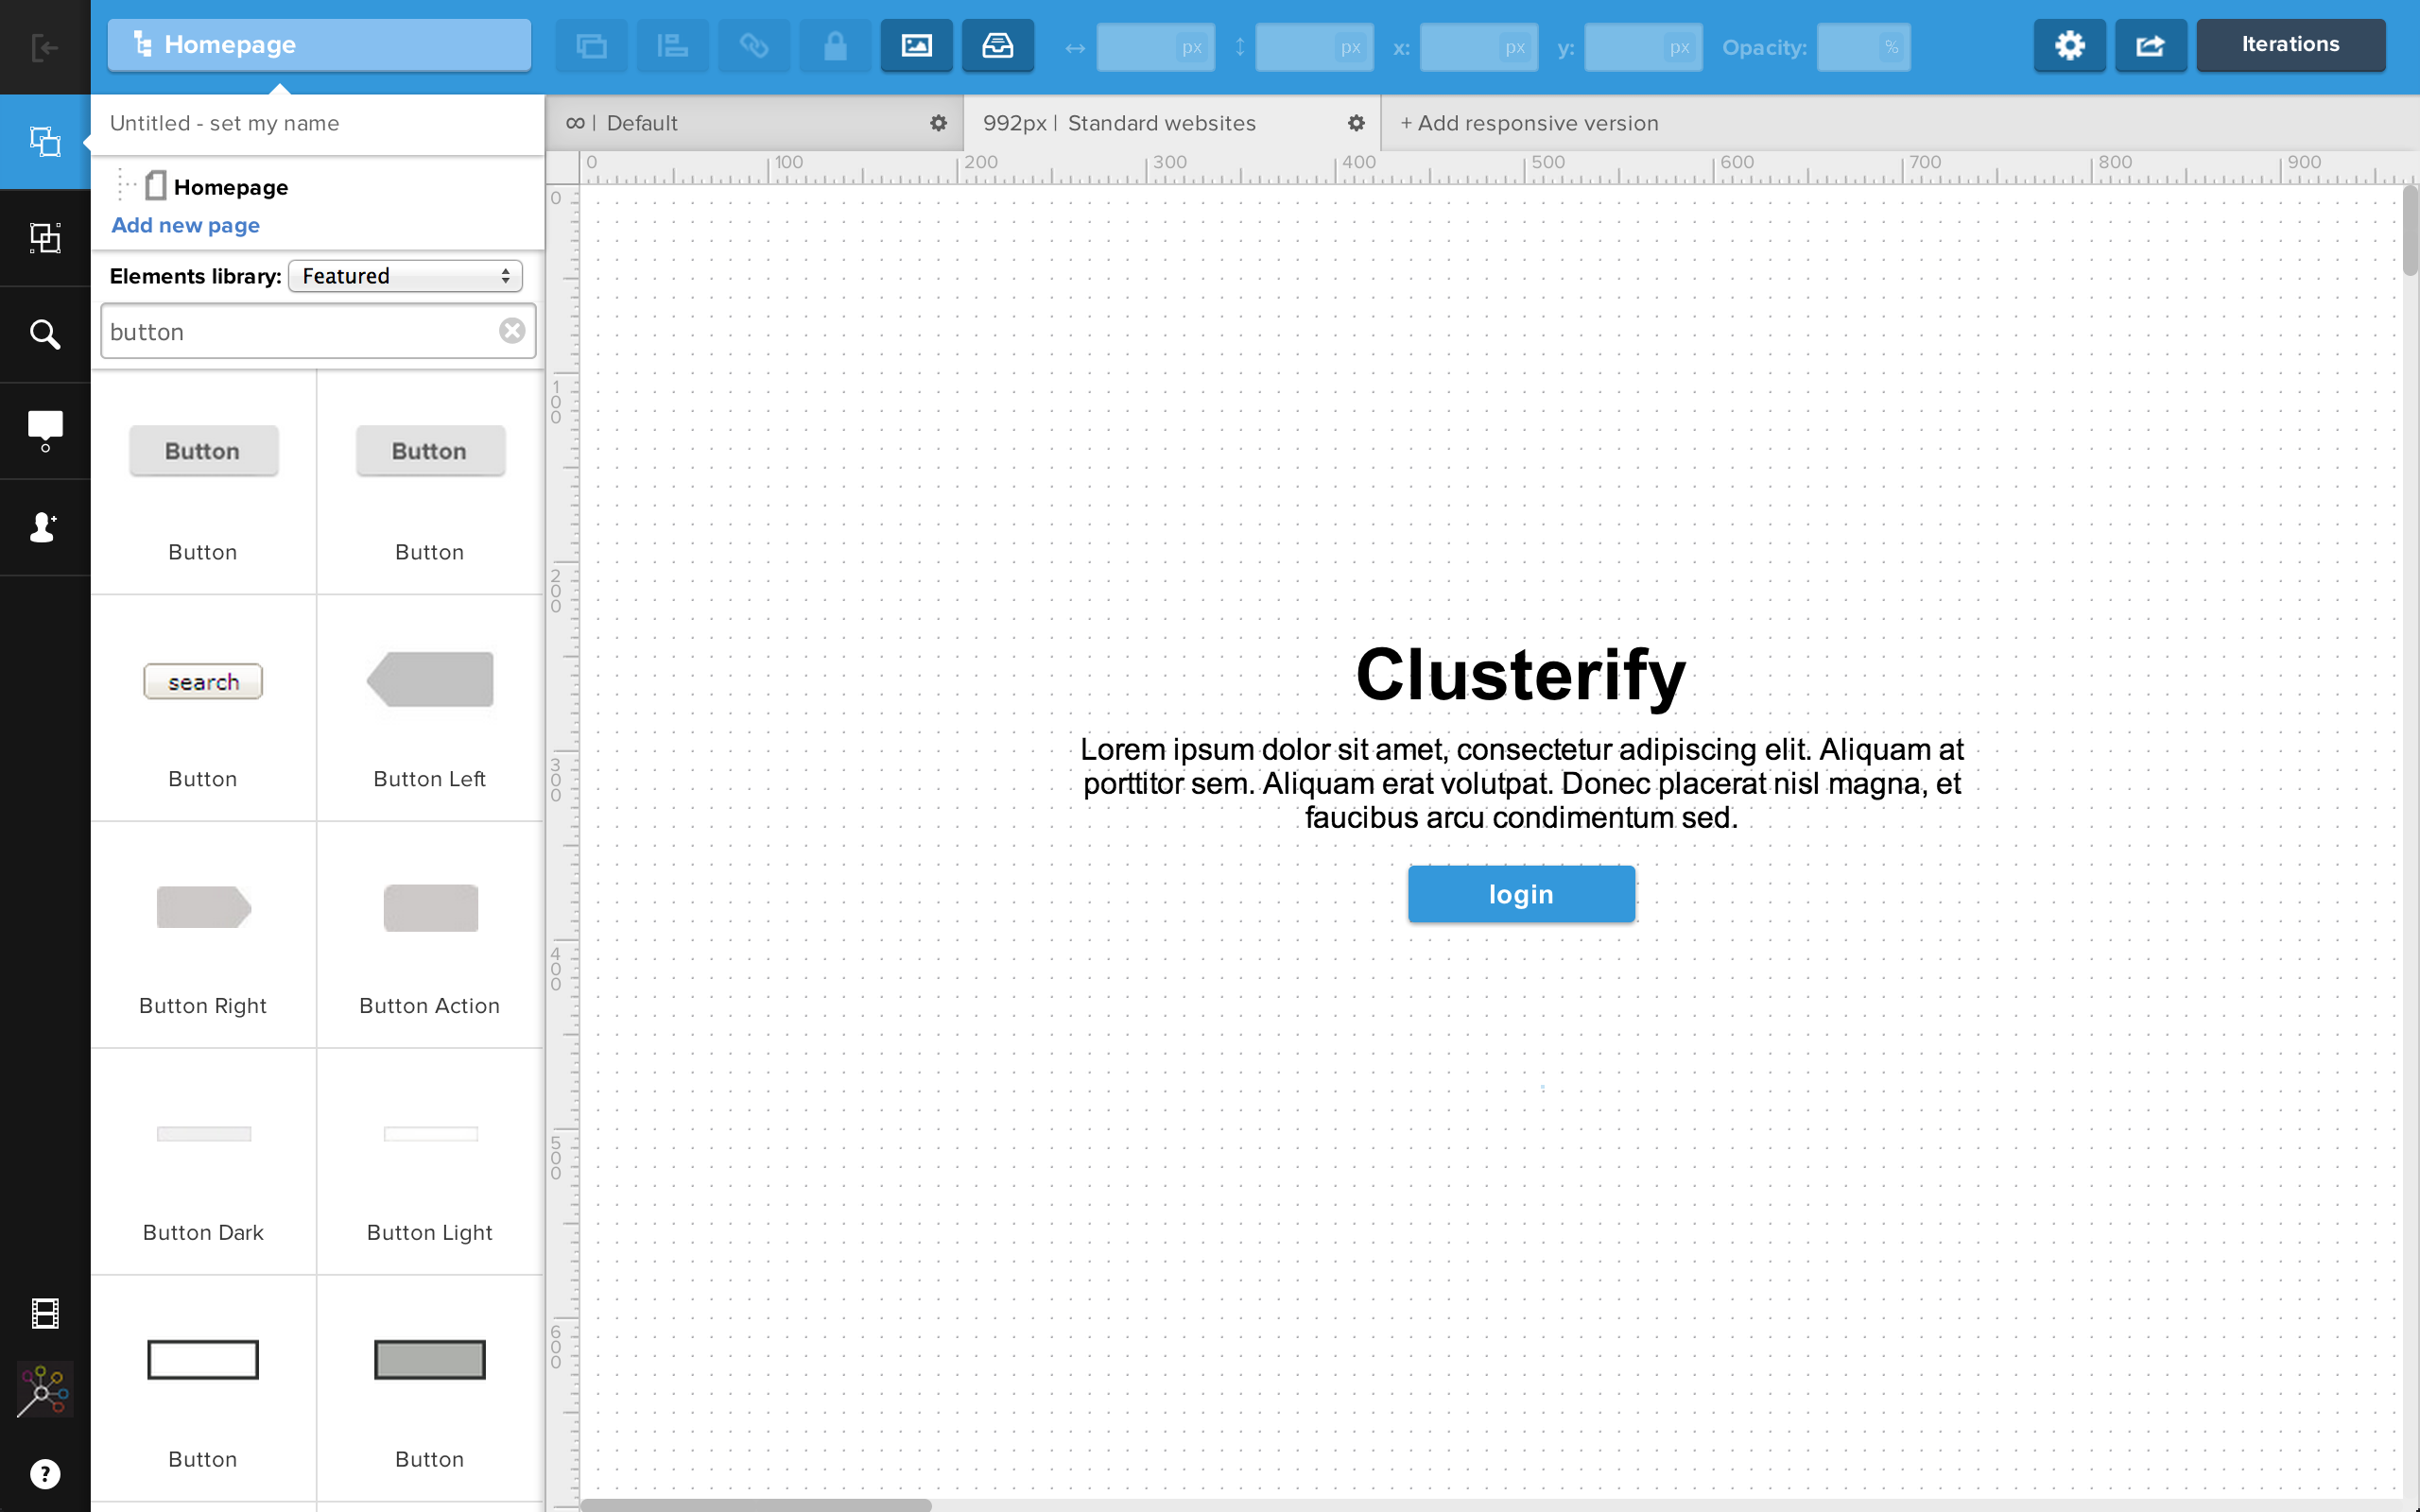
\includegraphics[width=\textwidth]{img/mockup/welcome.png}
        	\end{figure}

        	\begin{figure}[p]
		\textbf{Inserimento email}: pagina dove si richiederà di inserire la propria mail.\\

        		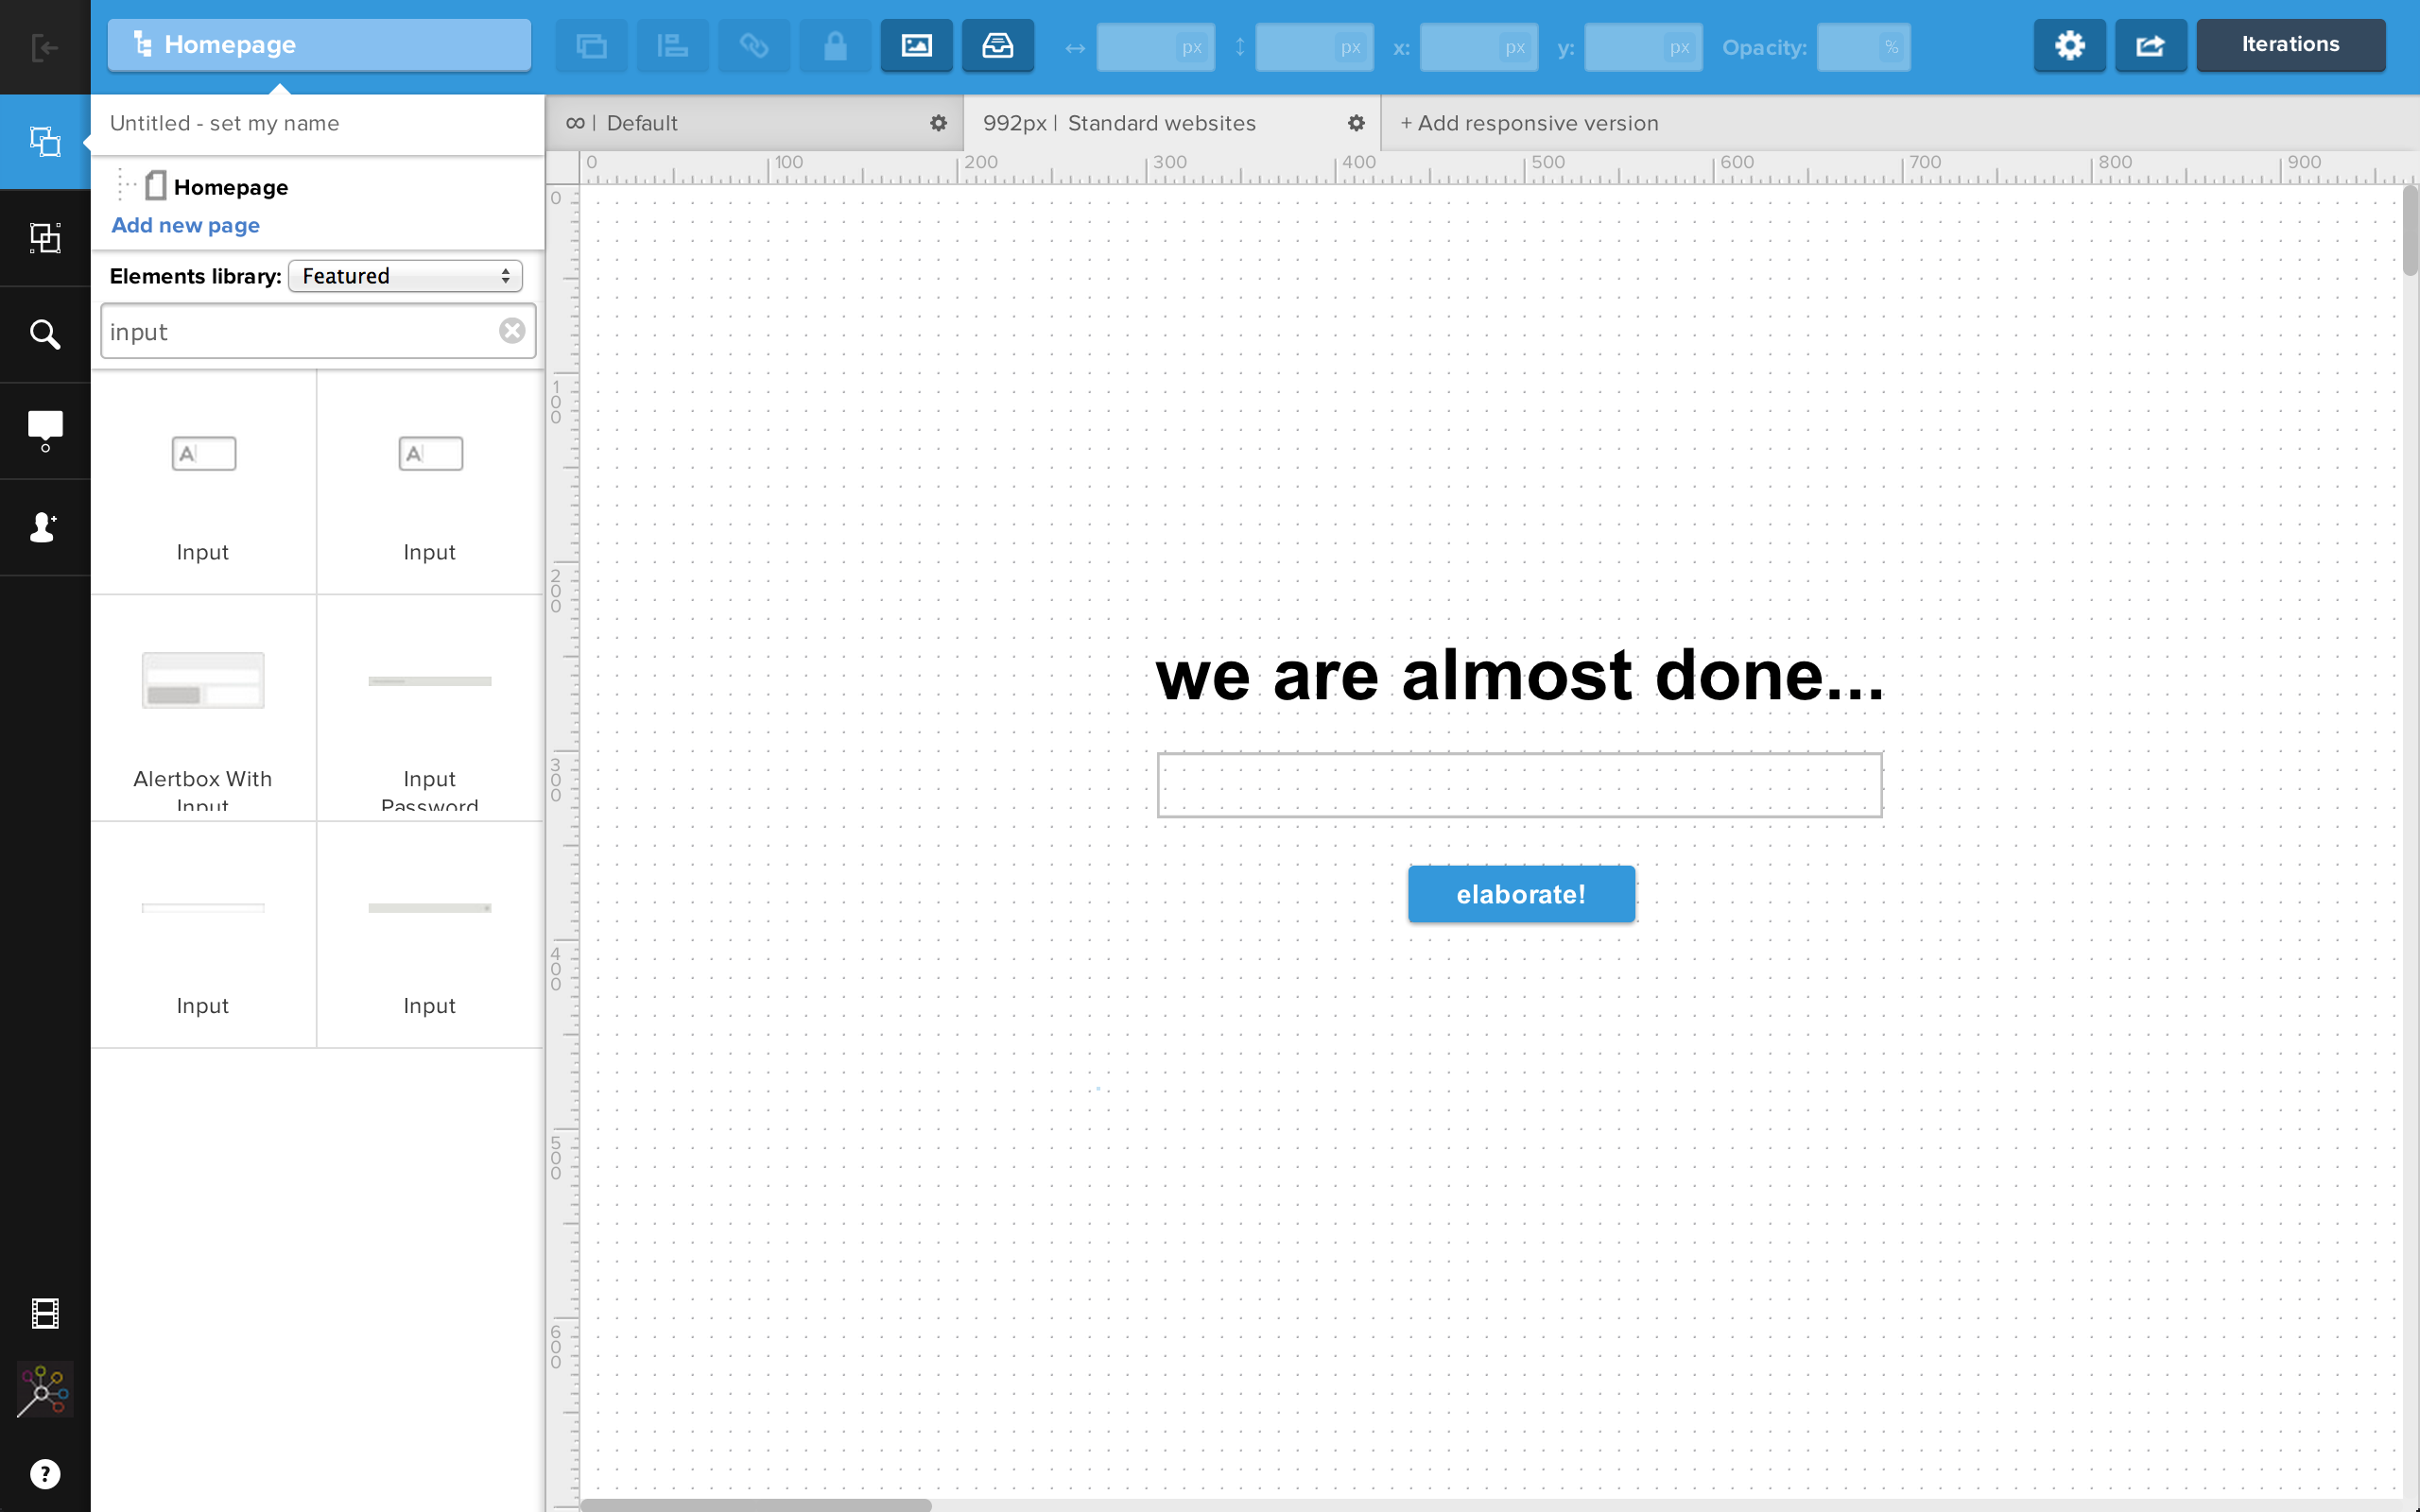
\includegraphics[width=\textwidth]{img/mockup/email.png}
        	\end{figure}

        	\begin{figure}[p]
		\textbf{Stato dell'elaborazione}: pagina che mostra all'utente lo stato dell'ultima elaborazione che questo ha lanciato.\\

        		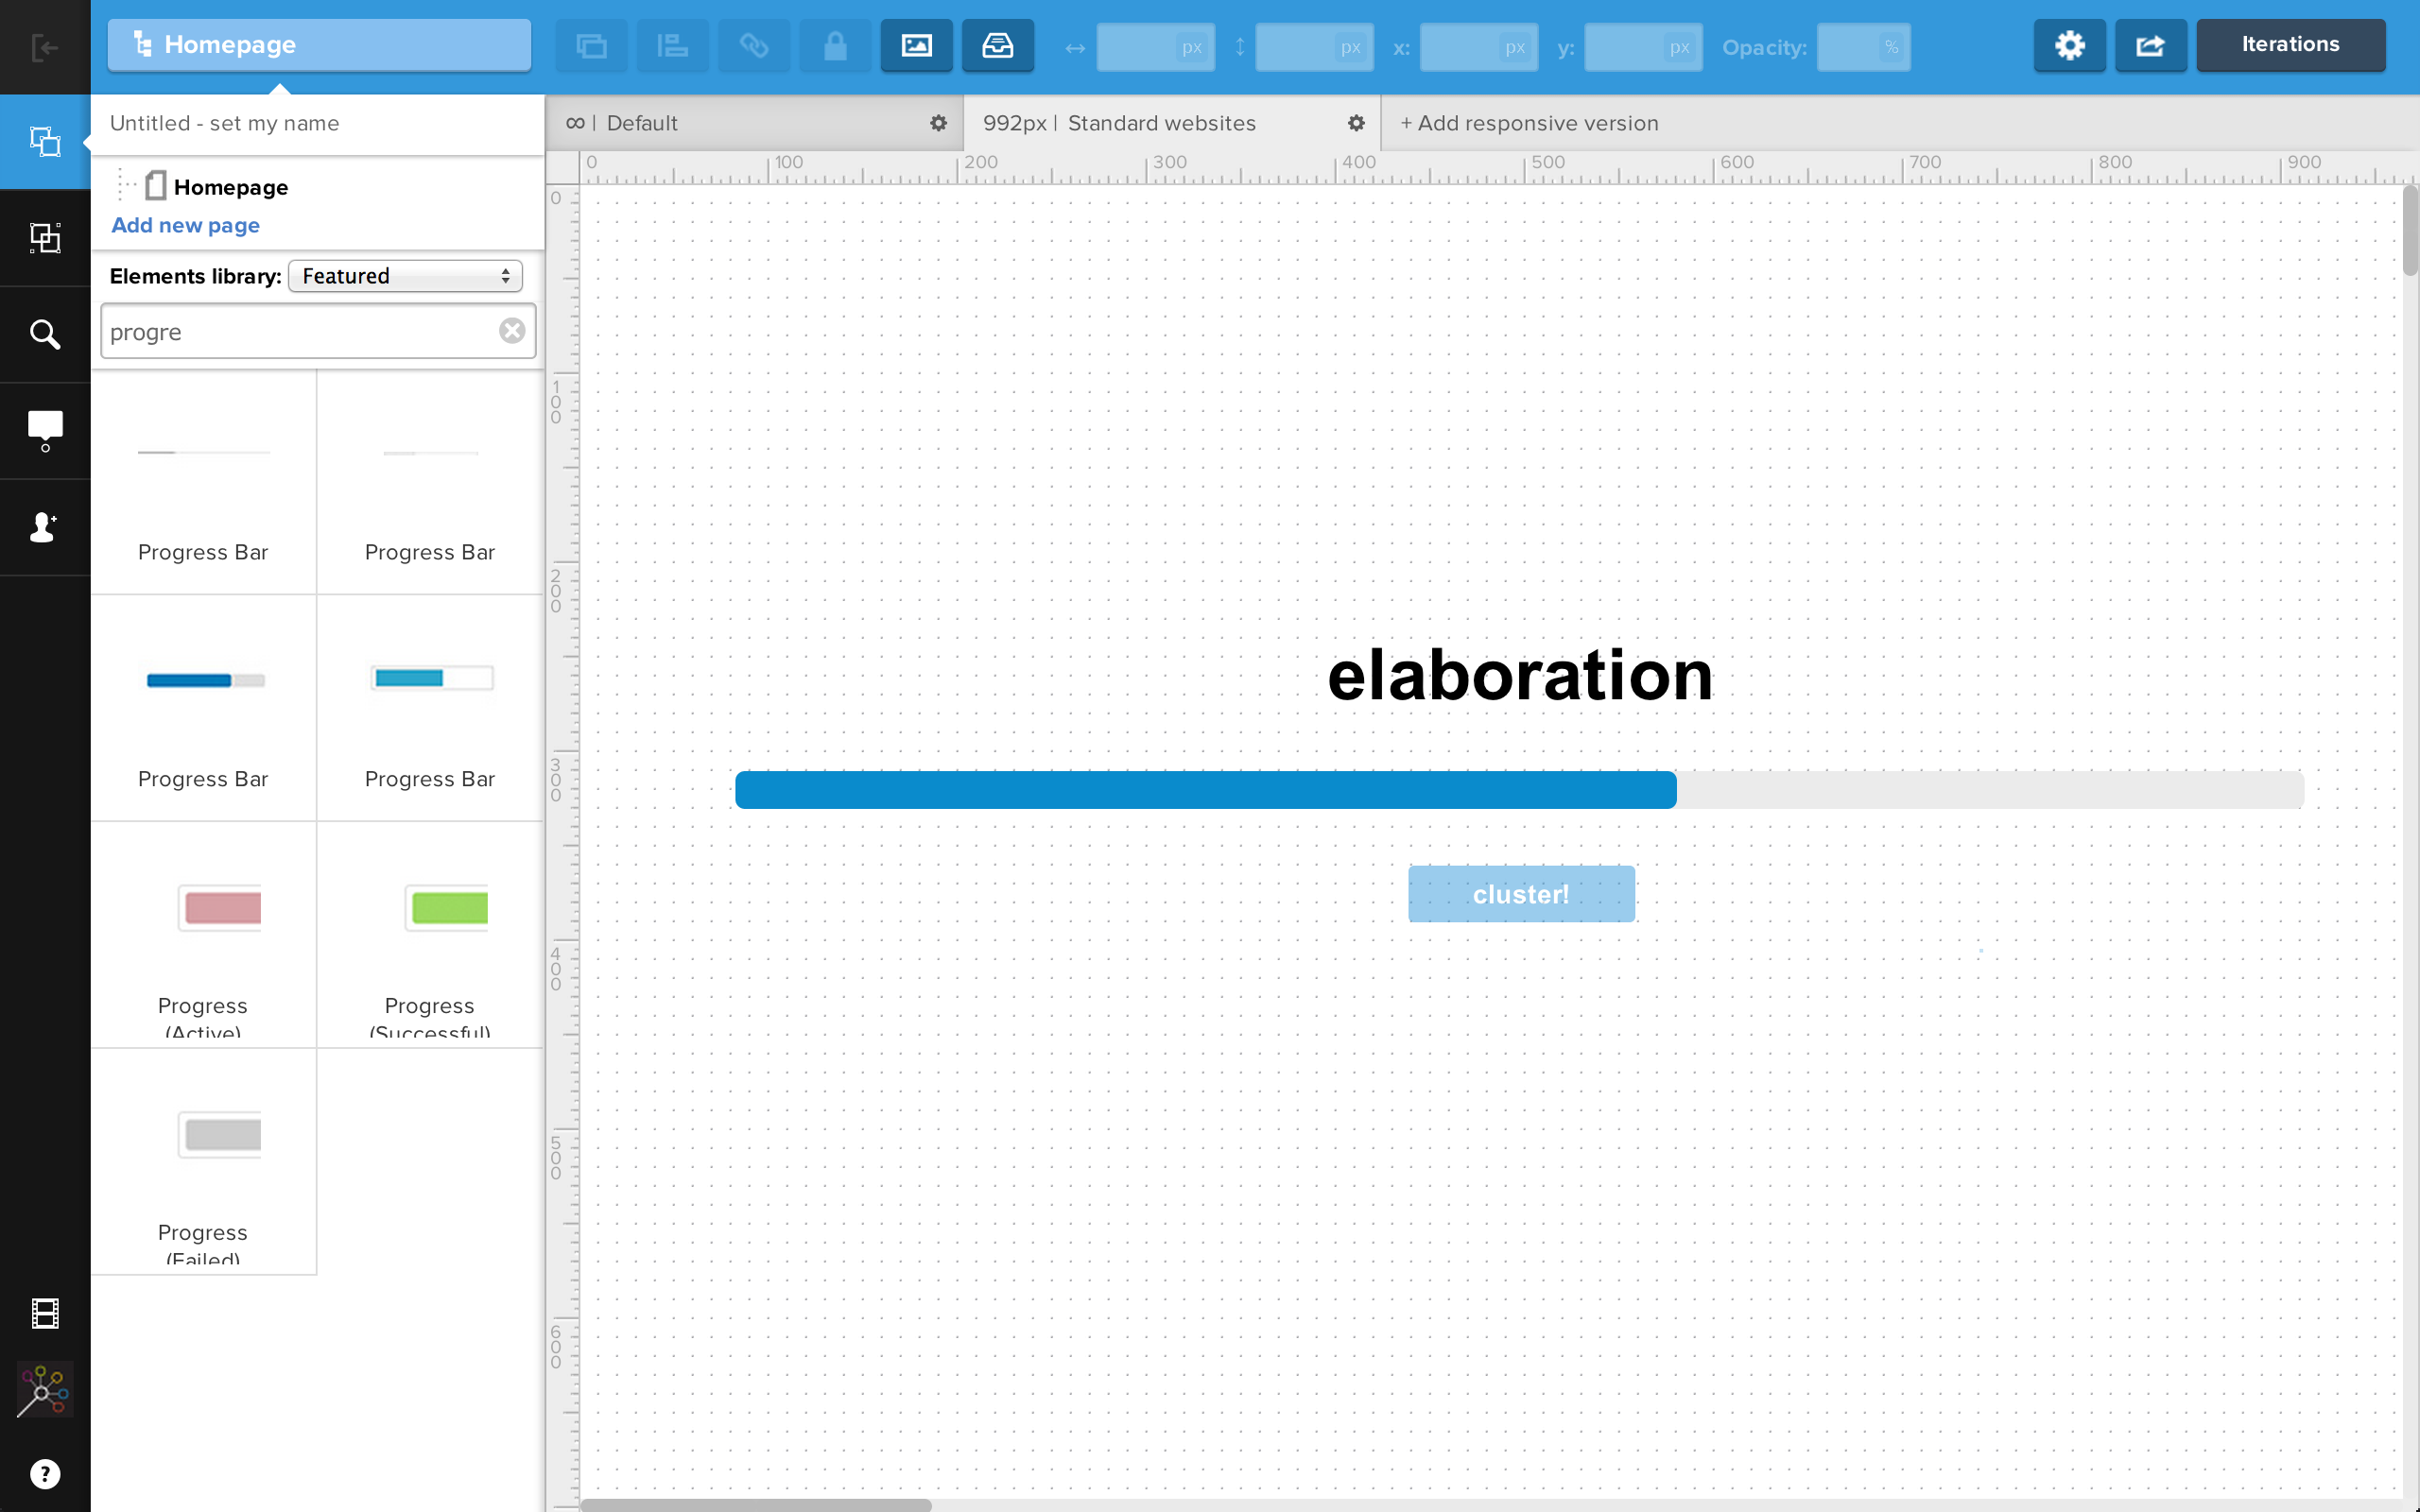
\includegraphics[width=\textwidth]{img/mockup/process.png}
        	\end{figure}

        	\begin{figure}[p]
		\textbf{Elaborazione}: pagina che mostra il risultato dell'elaborazione.\\

        		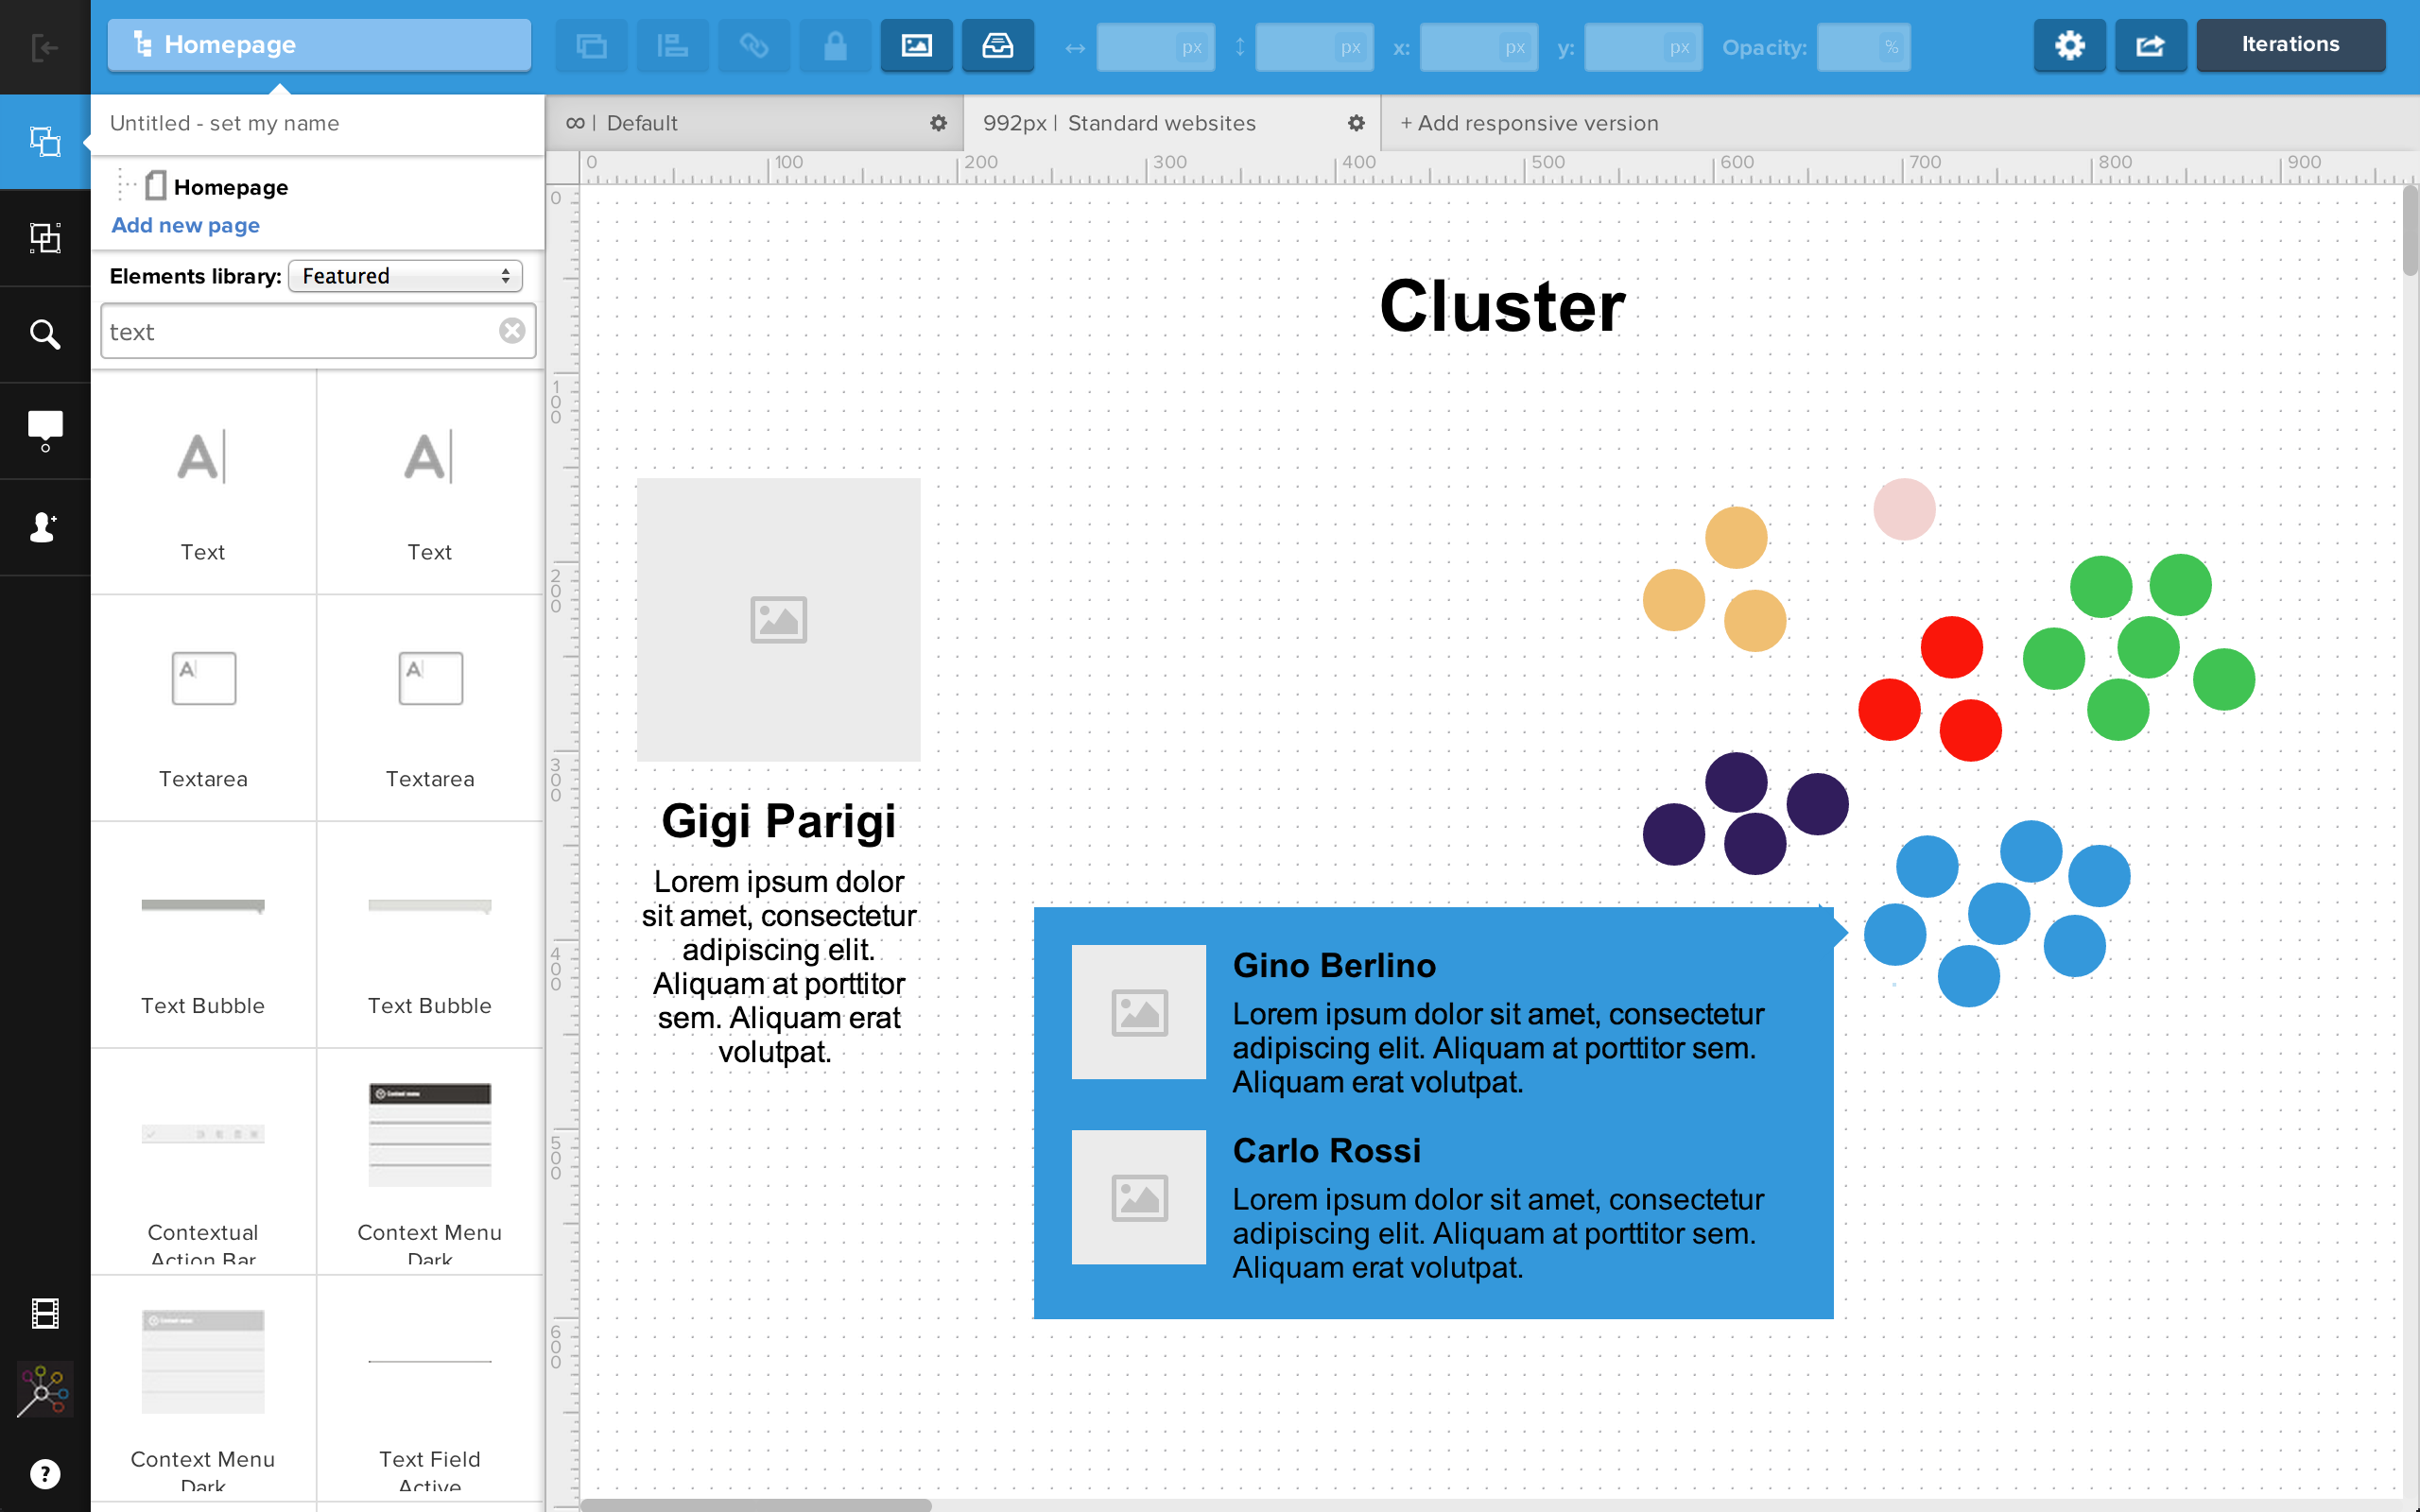
\includegraphics[width=\textwidth]{img/mockup/elaboration.png}
        	\end{figure}
            
	\newpage
         Questi mockup sono stati proposti a cinque utenti che hanno permesso di capire alcuni problemi che erano stati introdotti.
            
	\begin{itemize}
		\item  Nella pagina di richiesta dell'email non si capiva cosa venisse chiesto agli utenti. Si è deciso di aggiungere degli aiuti visivi che permetteranno loro di capire.
            
            	\item Nella pagina dedicata allo stato dell'elaborazione, gli intervistati non capivano cosa Clusterify stesse facendo, nemmeno che questo processo sarebbe continuato anche se loro avessero chiuso la pagina e che un'email gli avrebbe notificati quando questo sarebbe finito. Si è deciso di aggiungere una scritta che chiarirà il comportamento di Clusterify. 
                        
            	\item Nella pagina dedicata alla visualizzazione del cluster, viene dato poco spazio ai tweet mentre questi dovrebbero essere l'elemento fondamentale della piattaforma.
            
            	\item Si è notata la necessità di avere una pagina con le elaborazioni passate.
            \end{itemize}
            

\subsection{Studio finale}        
	Clusterify utilizza come framework di base Bootstrap -- \url{http://getbootstrap.com/} --, utile per alcune componenti quali la griglia ed i menù \emph{dropdown}.
        
	Per la parte di \emph{data visualization} utilizzerà d3 -- \url{http://d3js.org/} --, una libreria scritta in JavaScript utile per maneggiare dati e permettere la loro visualizzazione.
        
	Dopo aver capito i problemi riscontrati nei mockup dai primi intervistati, si è implementato Clusterify.

        	\begin{figure}[p]
		\textbf{Pagina di benvenuto}: landing page che offre la possibilità di registrarsi o di effettuare log in. Questa è anche la pagina dove si viene ridirezionati quando si richiede una visualizzazione di una pagina bloccata.\\

        		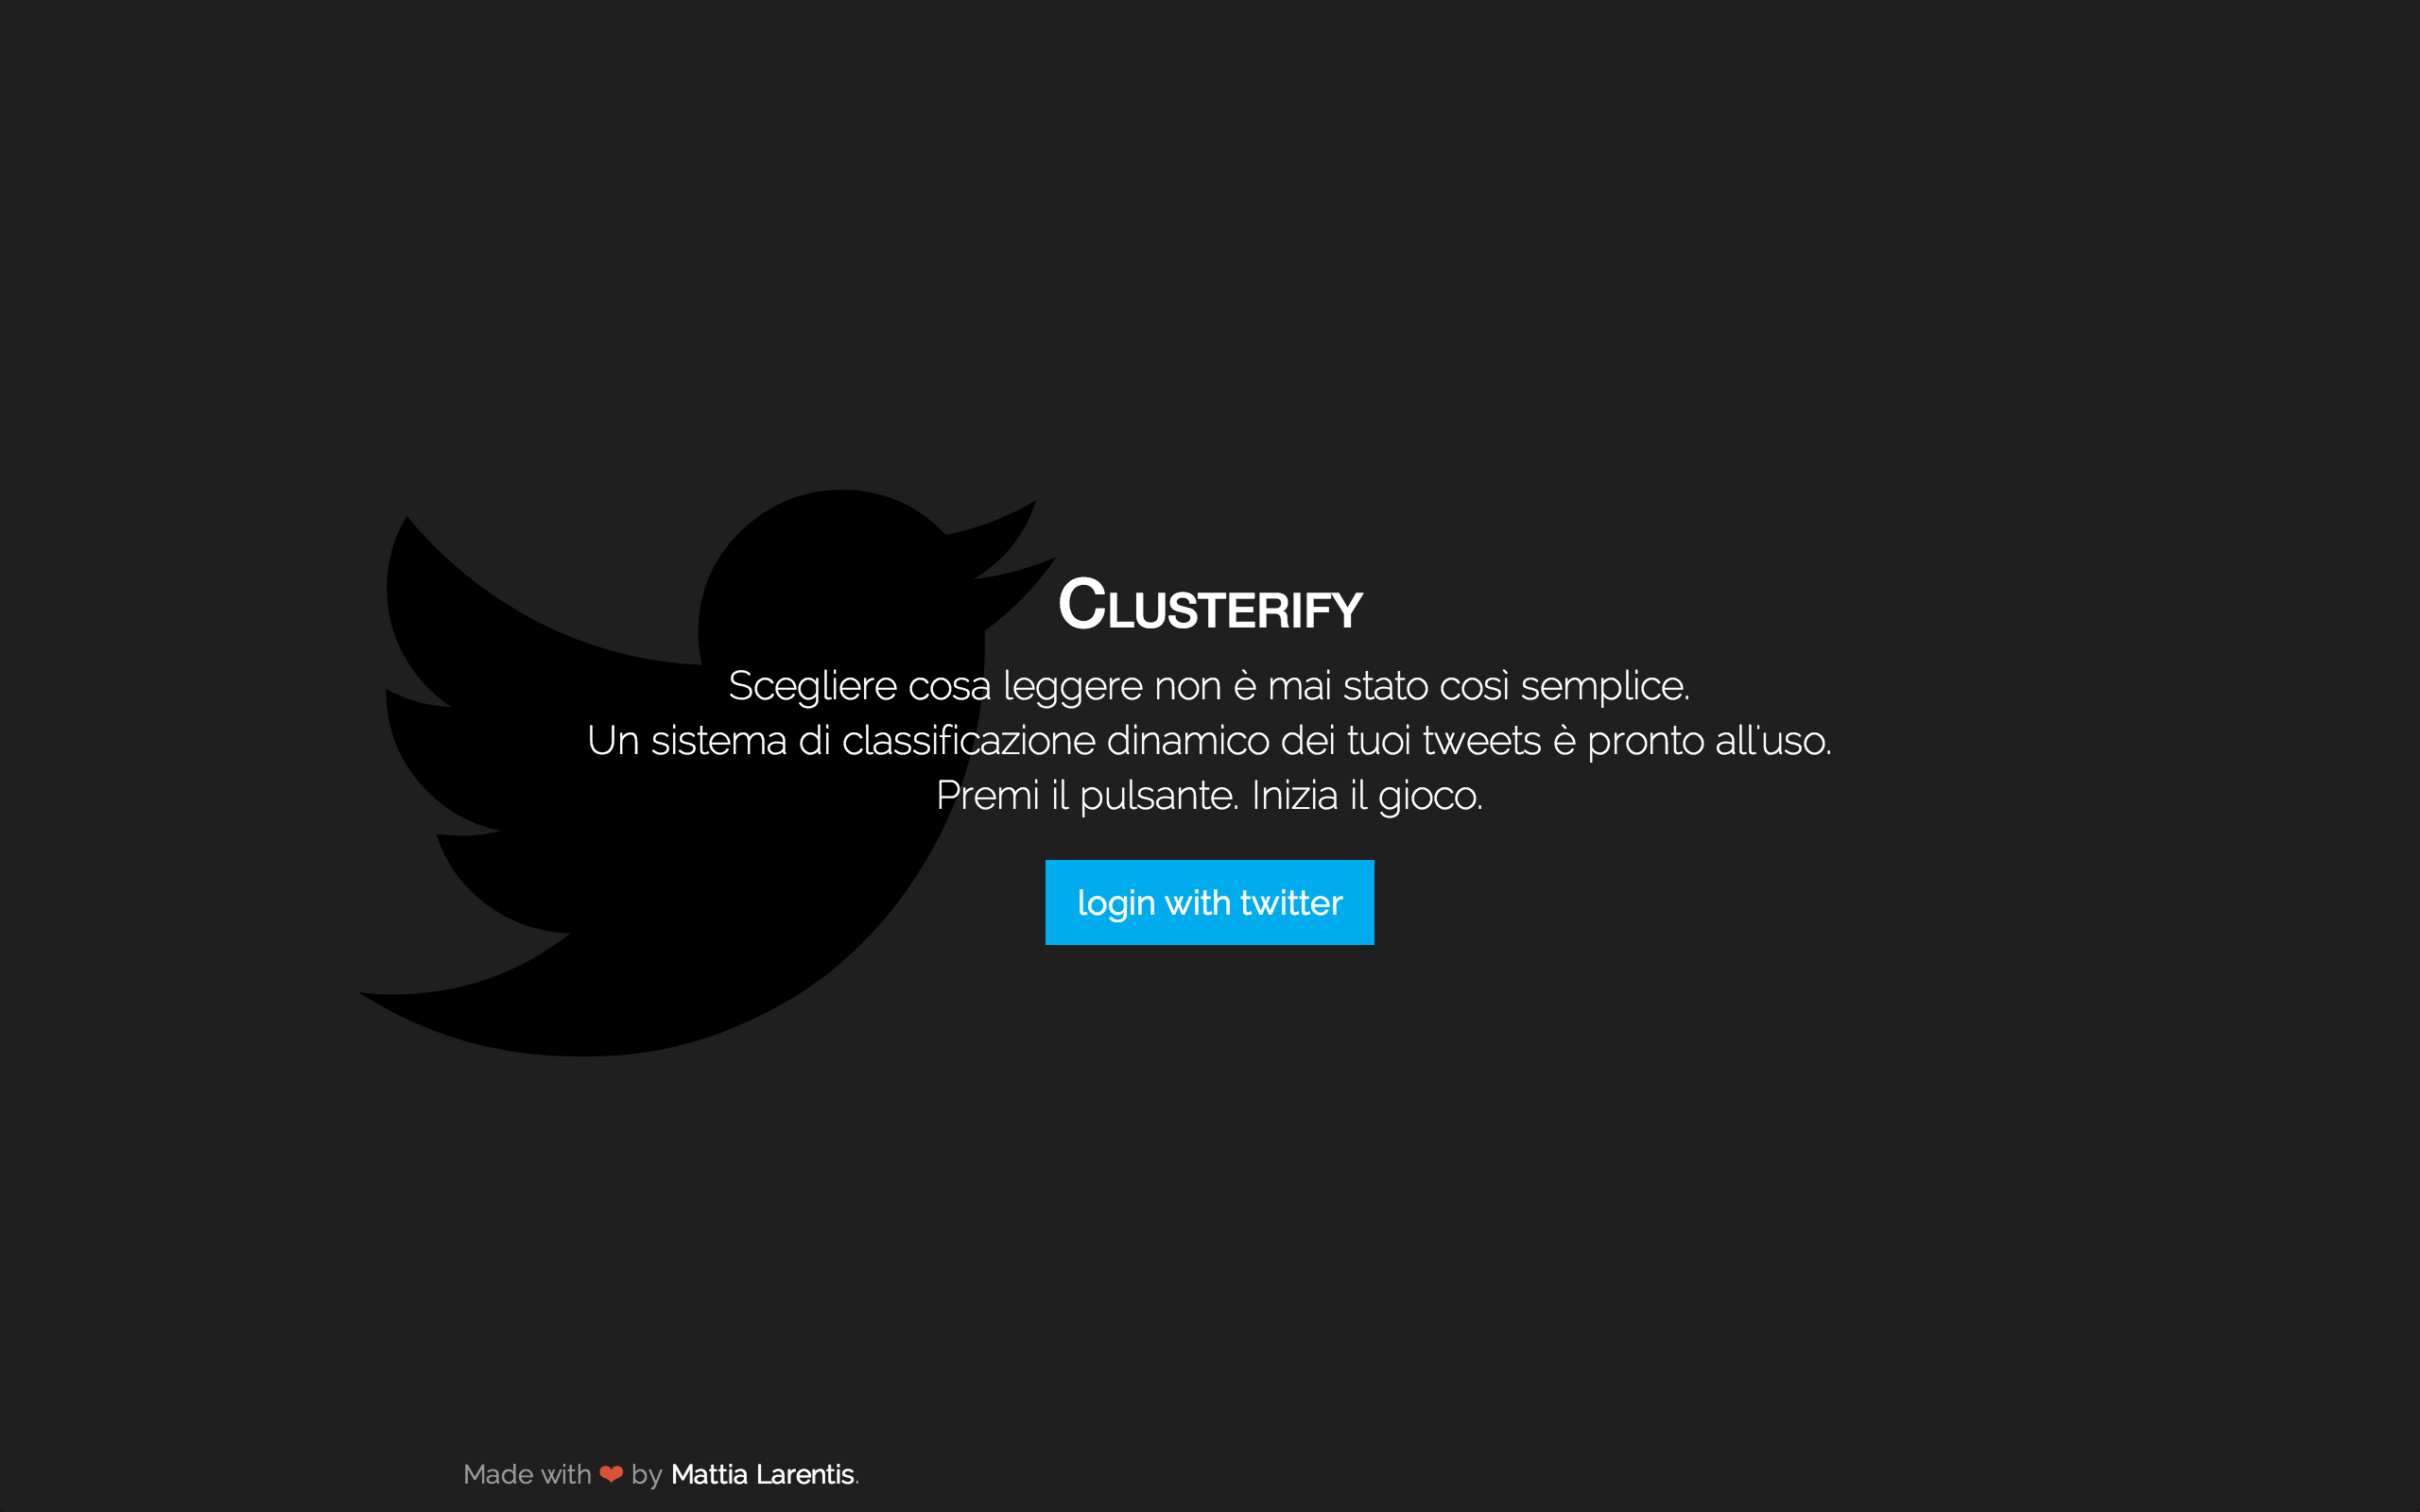
\includegraphics[width=\textwidth]{img/clusterify/welcome.png}
        	\end{figure}
        
        	\begin{figure}[p]
		\textbf{Inserimento email}: nel momento in cui un utente si registra, viene domandato di inserire una propria email. L'indirizzo è necessario per contattare l'utente quando un'elaborazione termina.\\

        		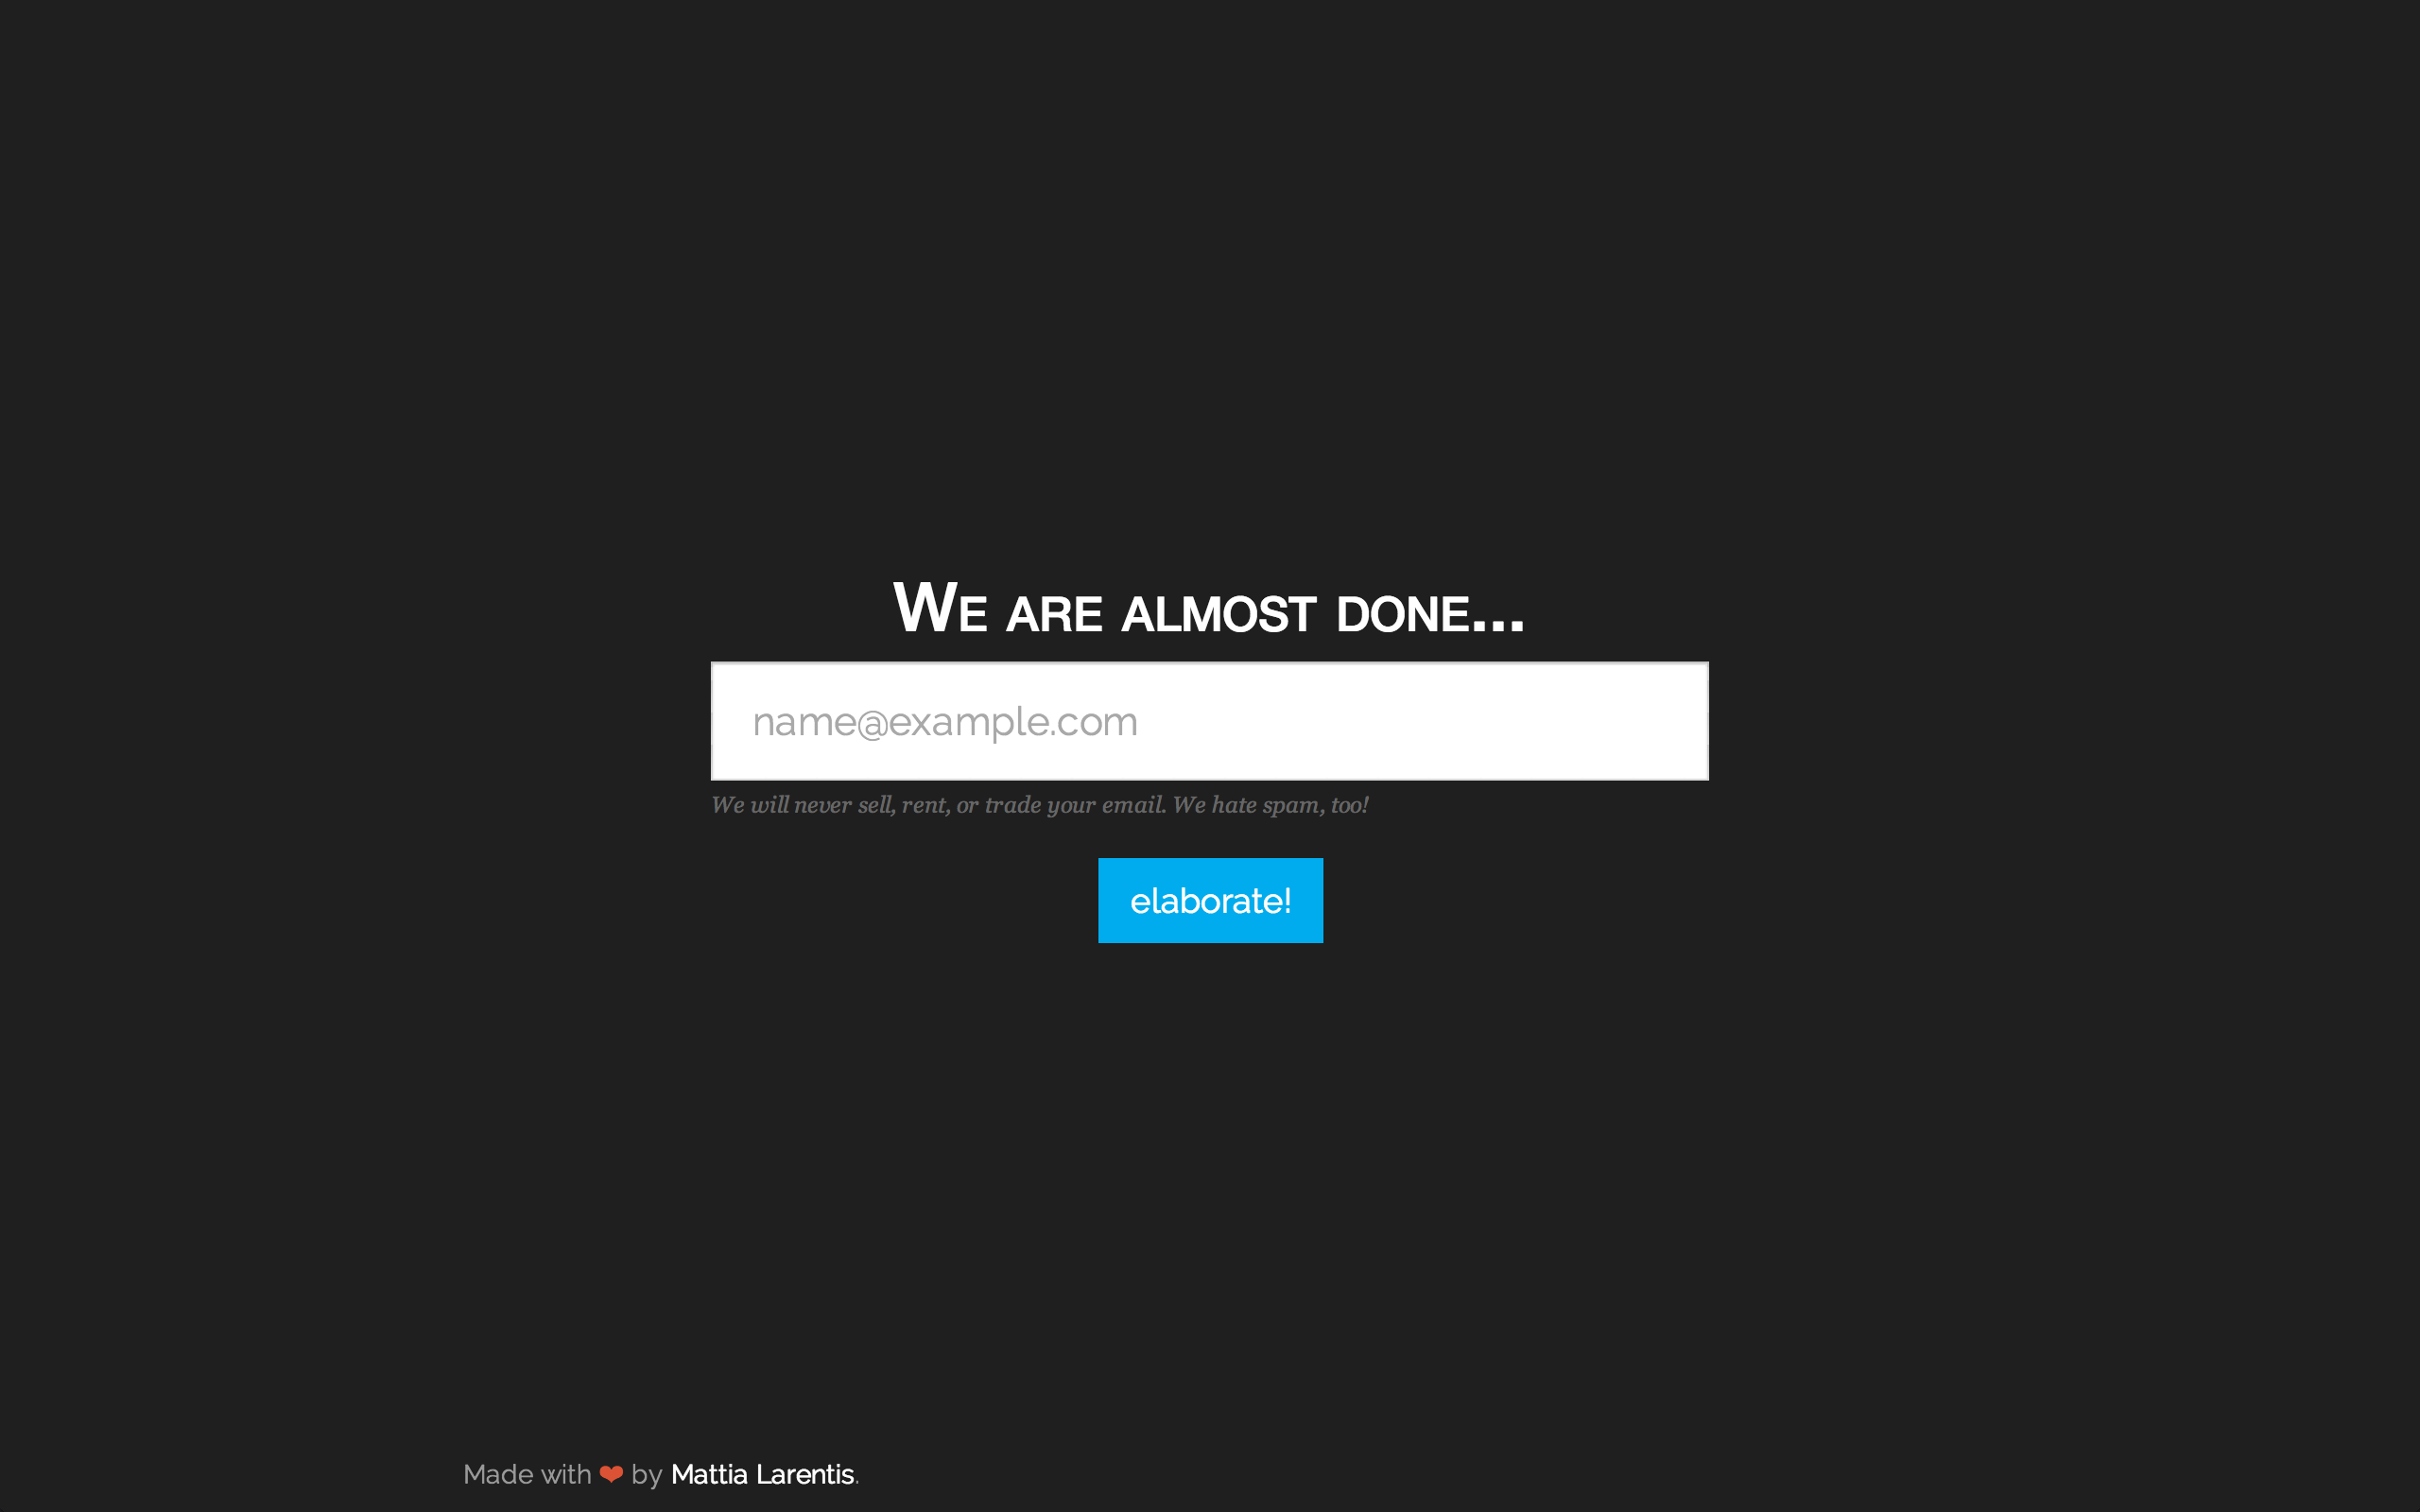
\includegraphics[width=\textwidth]{img/clusterify/email.png}
        	\end{figure}
        
        	\begin{figure}[p]
		\textbf{Stato dell'elaborazione}: quando un utente lancia un'elaborazione viene mostrata questa \emph{progress-bar}. La grafica segue passo a passo l'esecuzione del processo nel backend, illuminando la parte in corso.\\

        		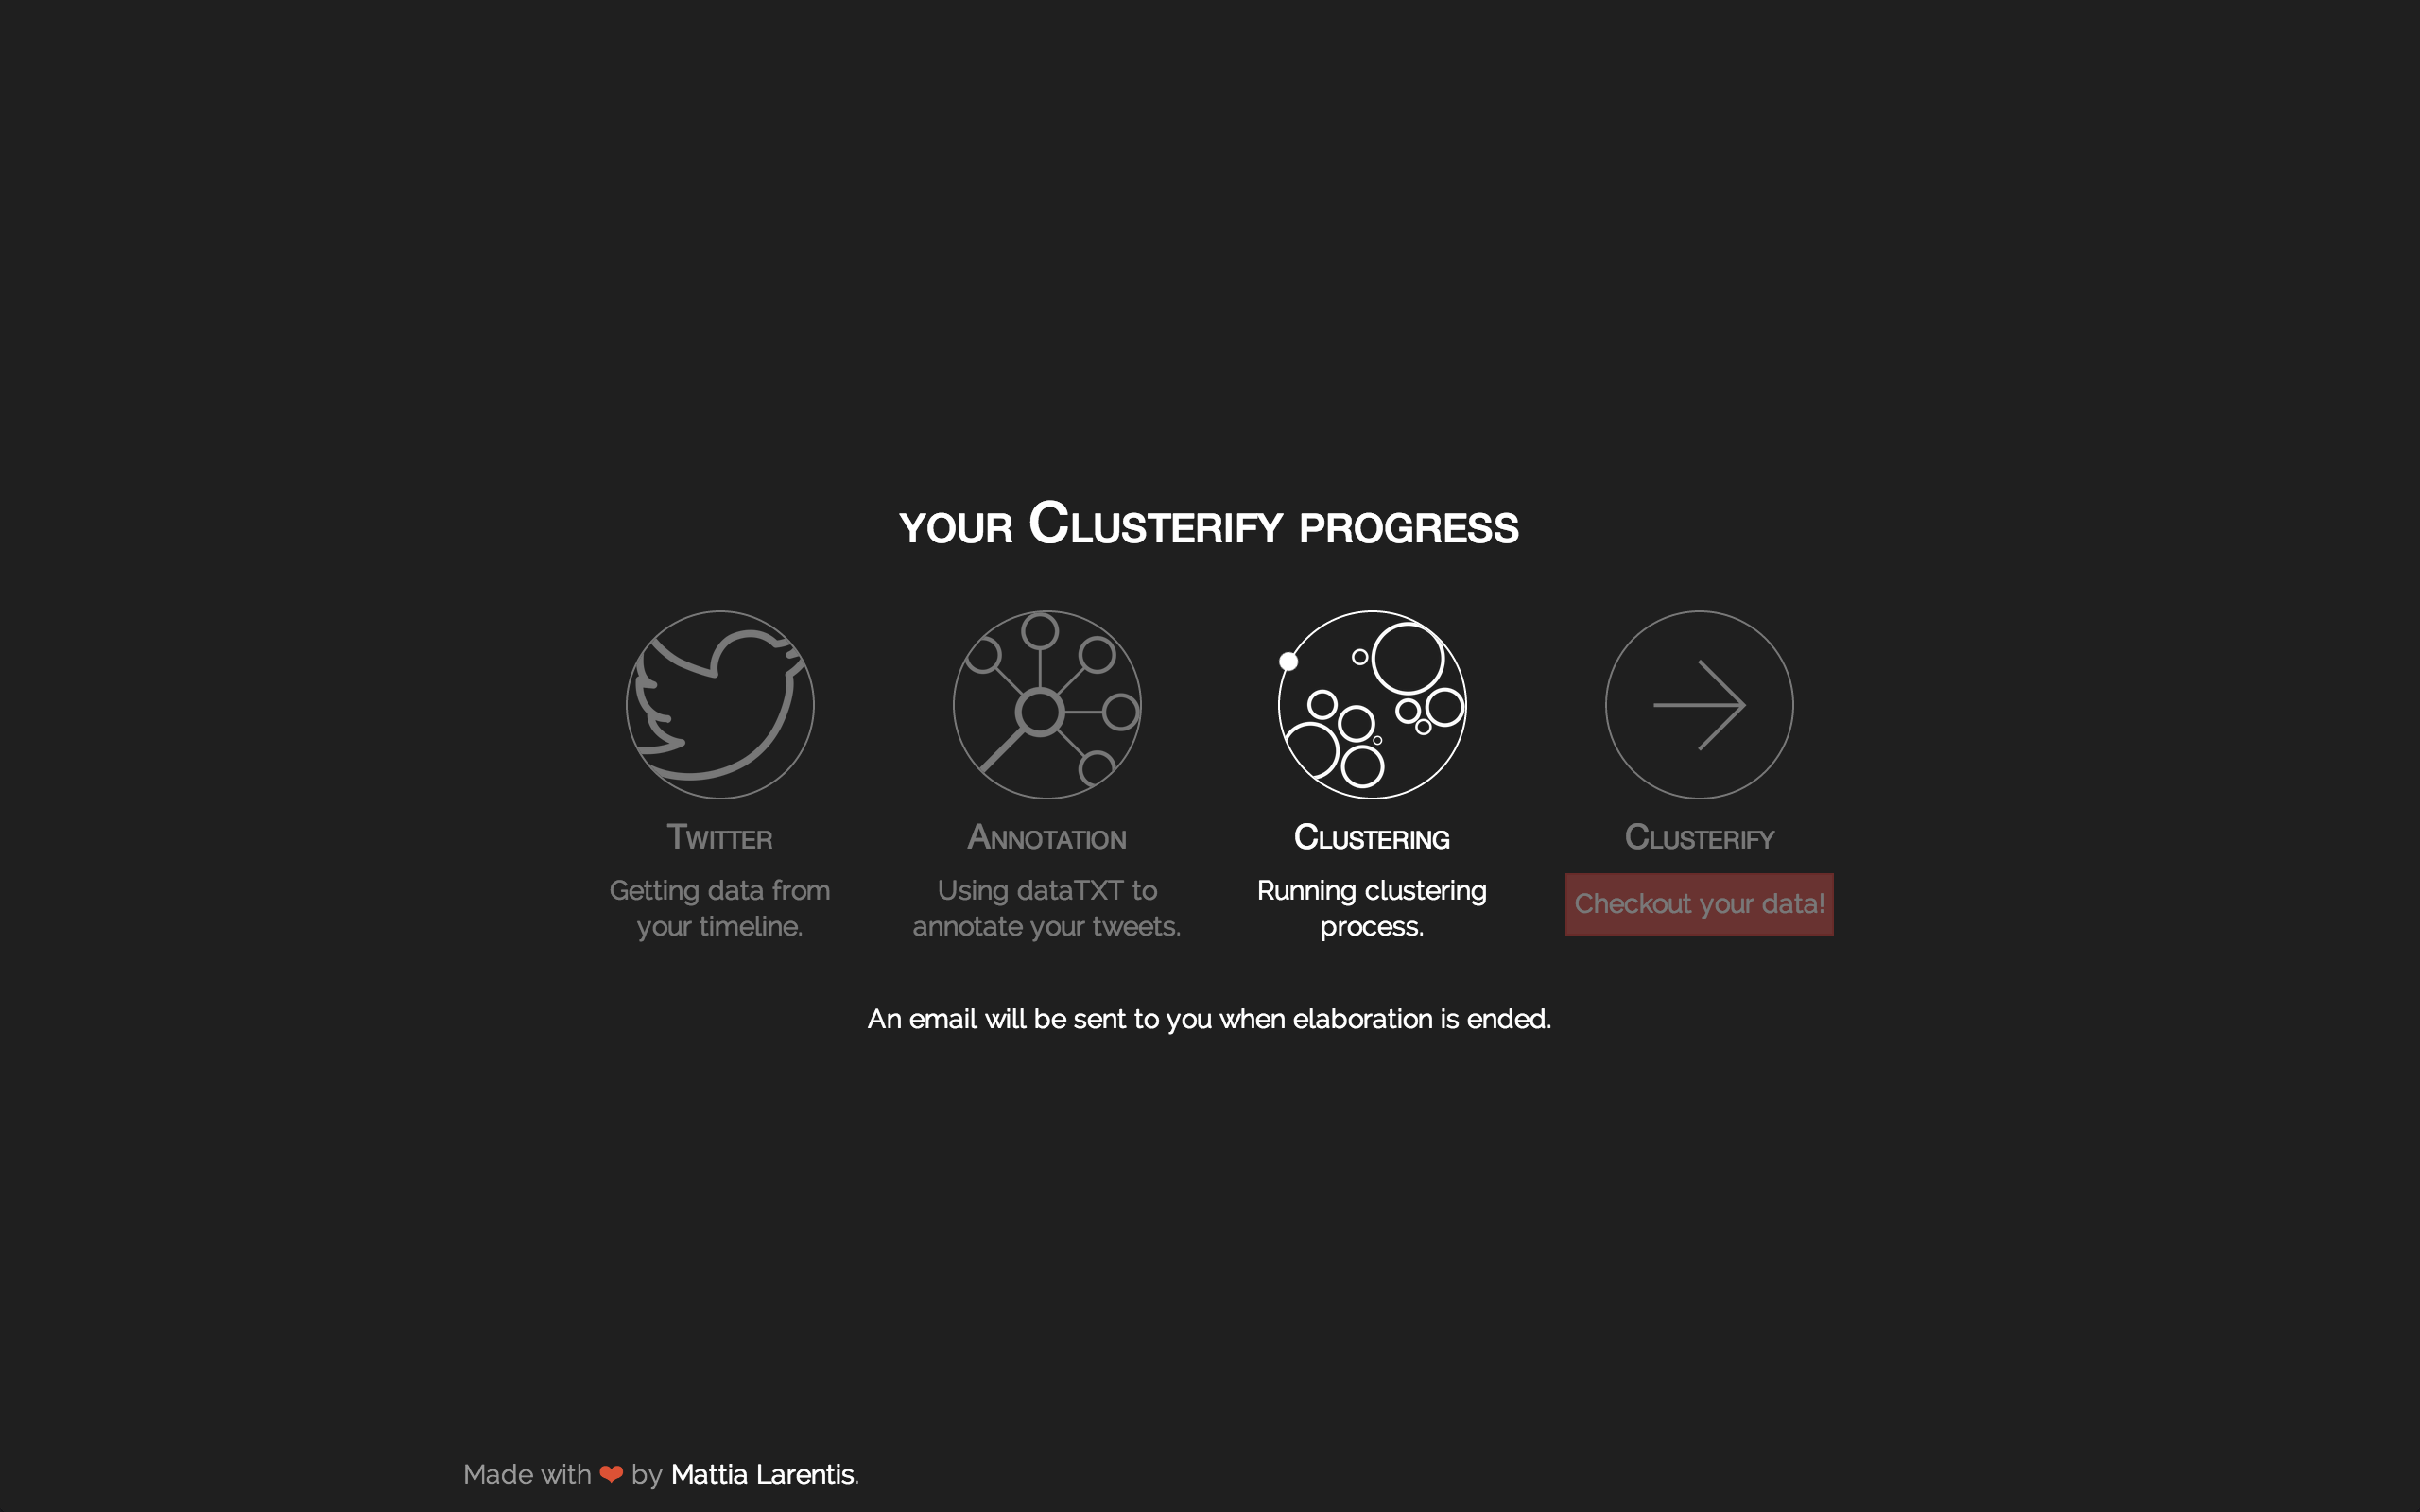
\includegraphics[width=\textwidth]{img/clusterify/process.png}
        	\end{figure}
        
        	\begin{figure}[p]
		\textbf{Elaborazione}: pagina che mostra il cluster calcolato da Clusterify. Dal menù in alto è possibile lanciare una nuova elaborazione oppure visualizzare lo storico.\\

        		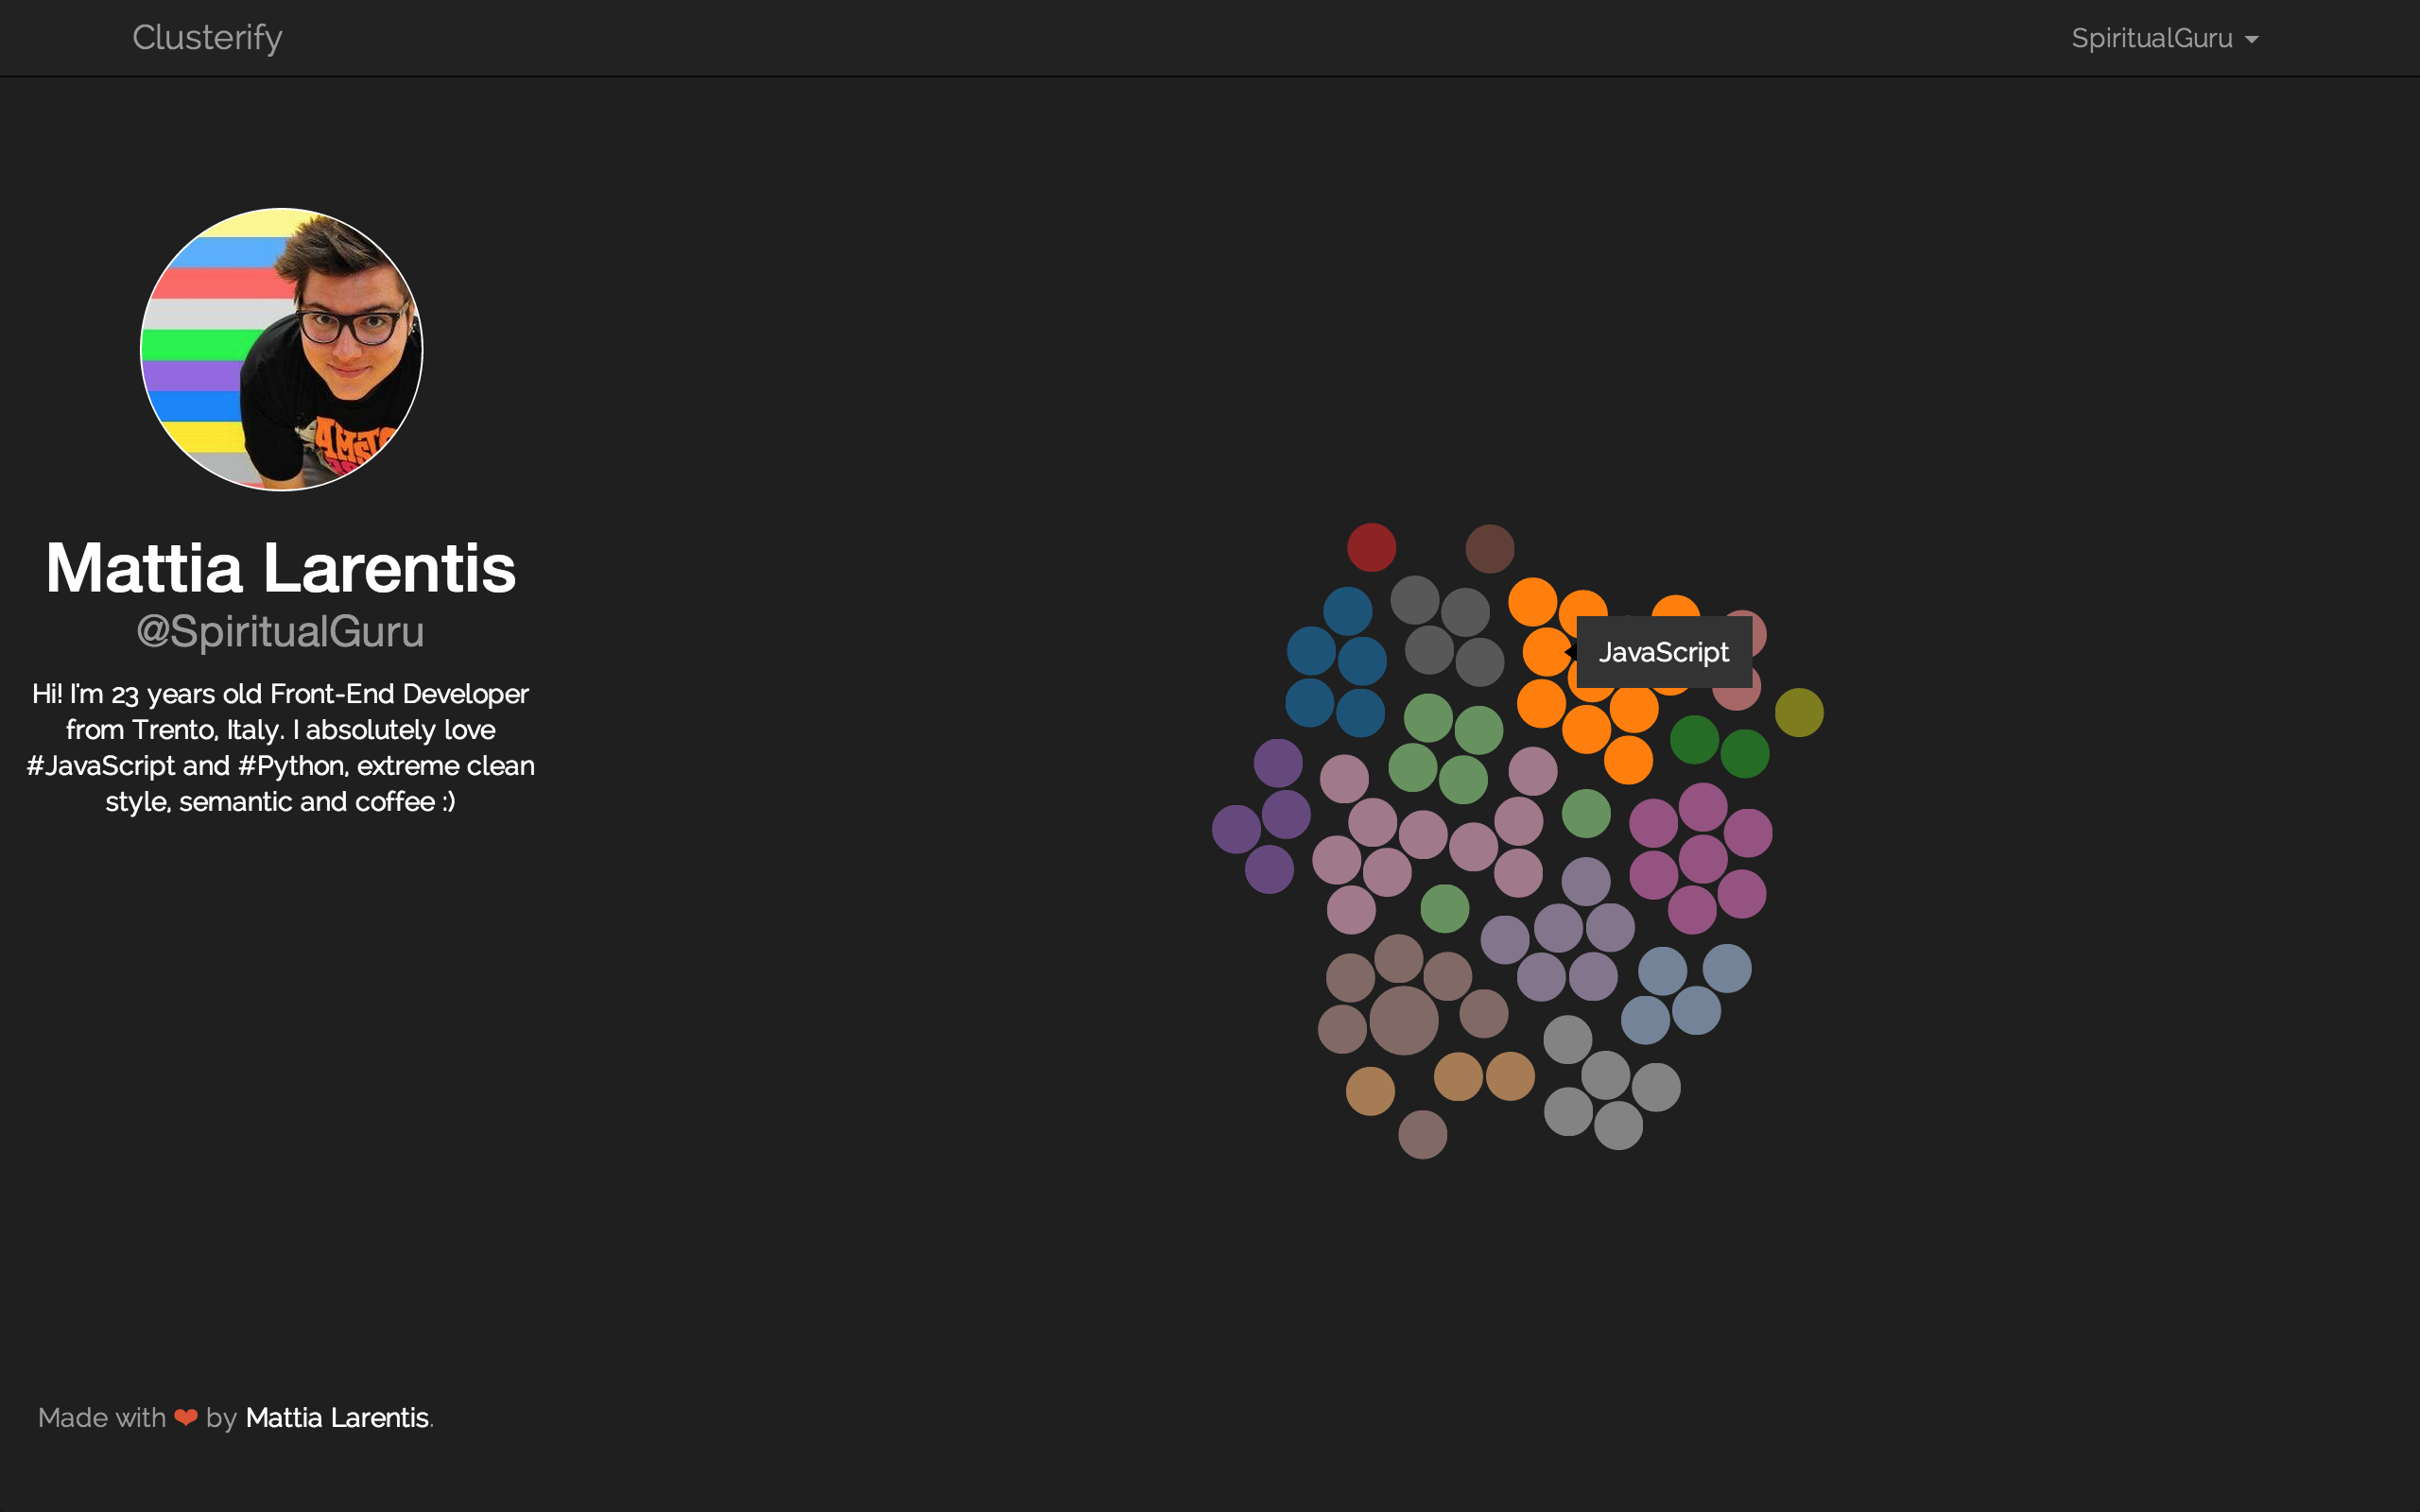
\includegraphics[width=\textwidth]{img/clusterify/elaboration.png}
        	\end{figure}
        
        	\begin{figure}[p]
		\textbf{Tweet}: da ``Elaborazione'' è possibile navigare ogni cluster clickando su un qualsiasi elemento che lo compone. Quando ciò succede, una finestra modale si apre e permette di leggere tutti i tweet che sono stati raggruppati. Un tweet può appartenere a più cluster. Se un tweet viene premuto, si viene mandati alla pagina di Twitter dove il tweet risiede.\\

        		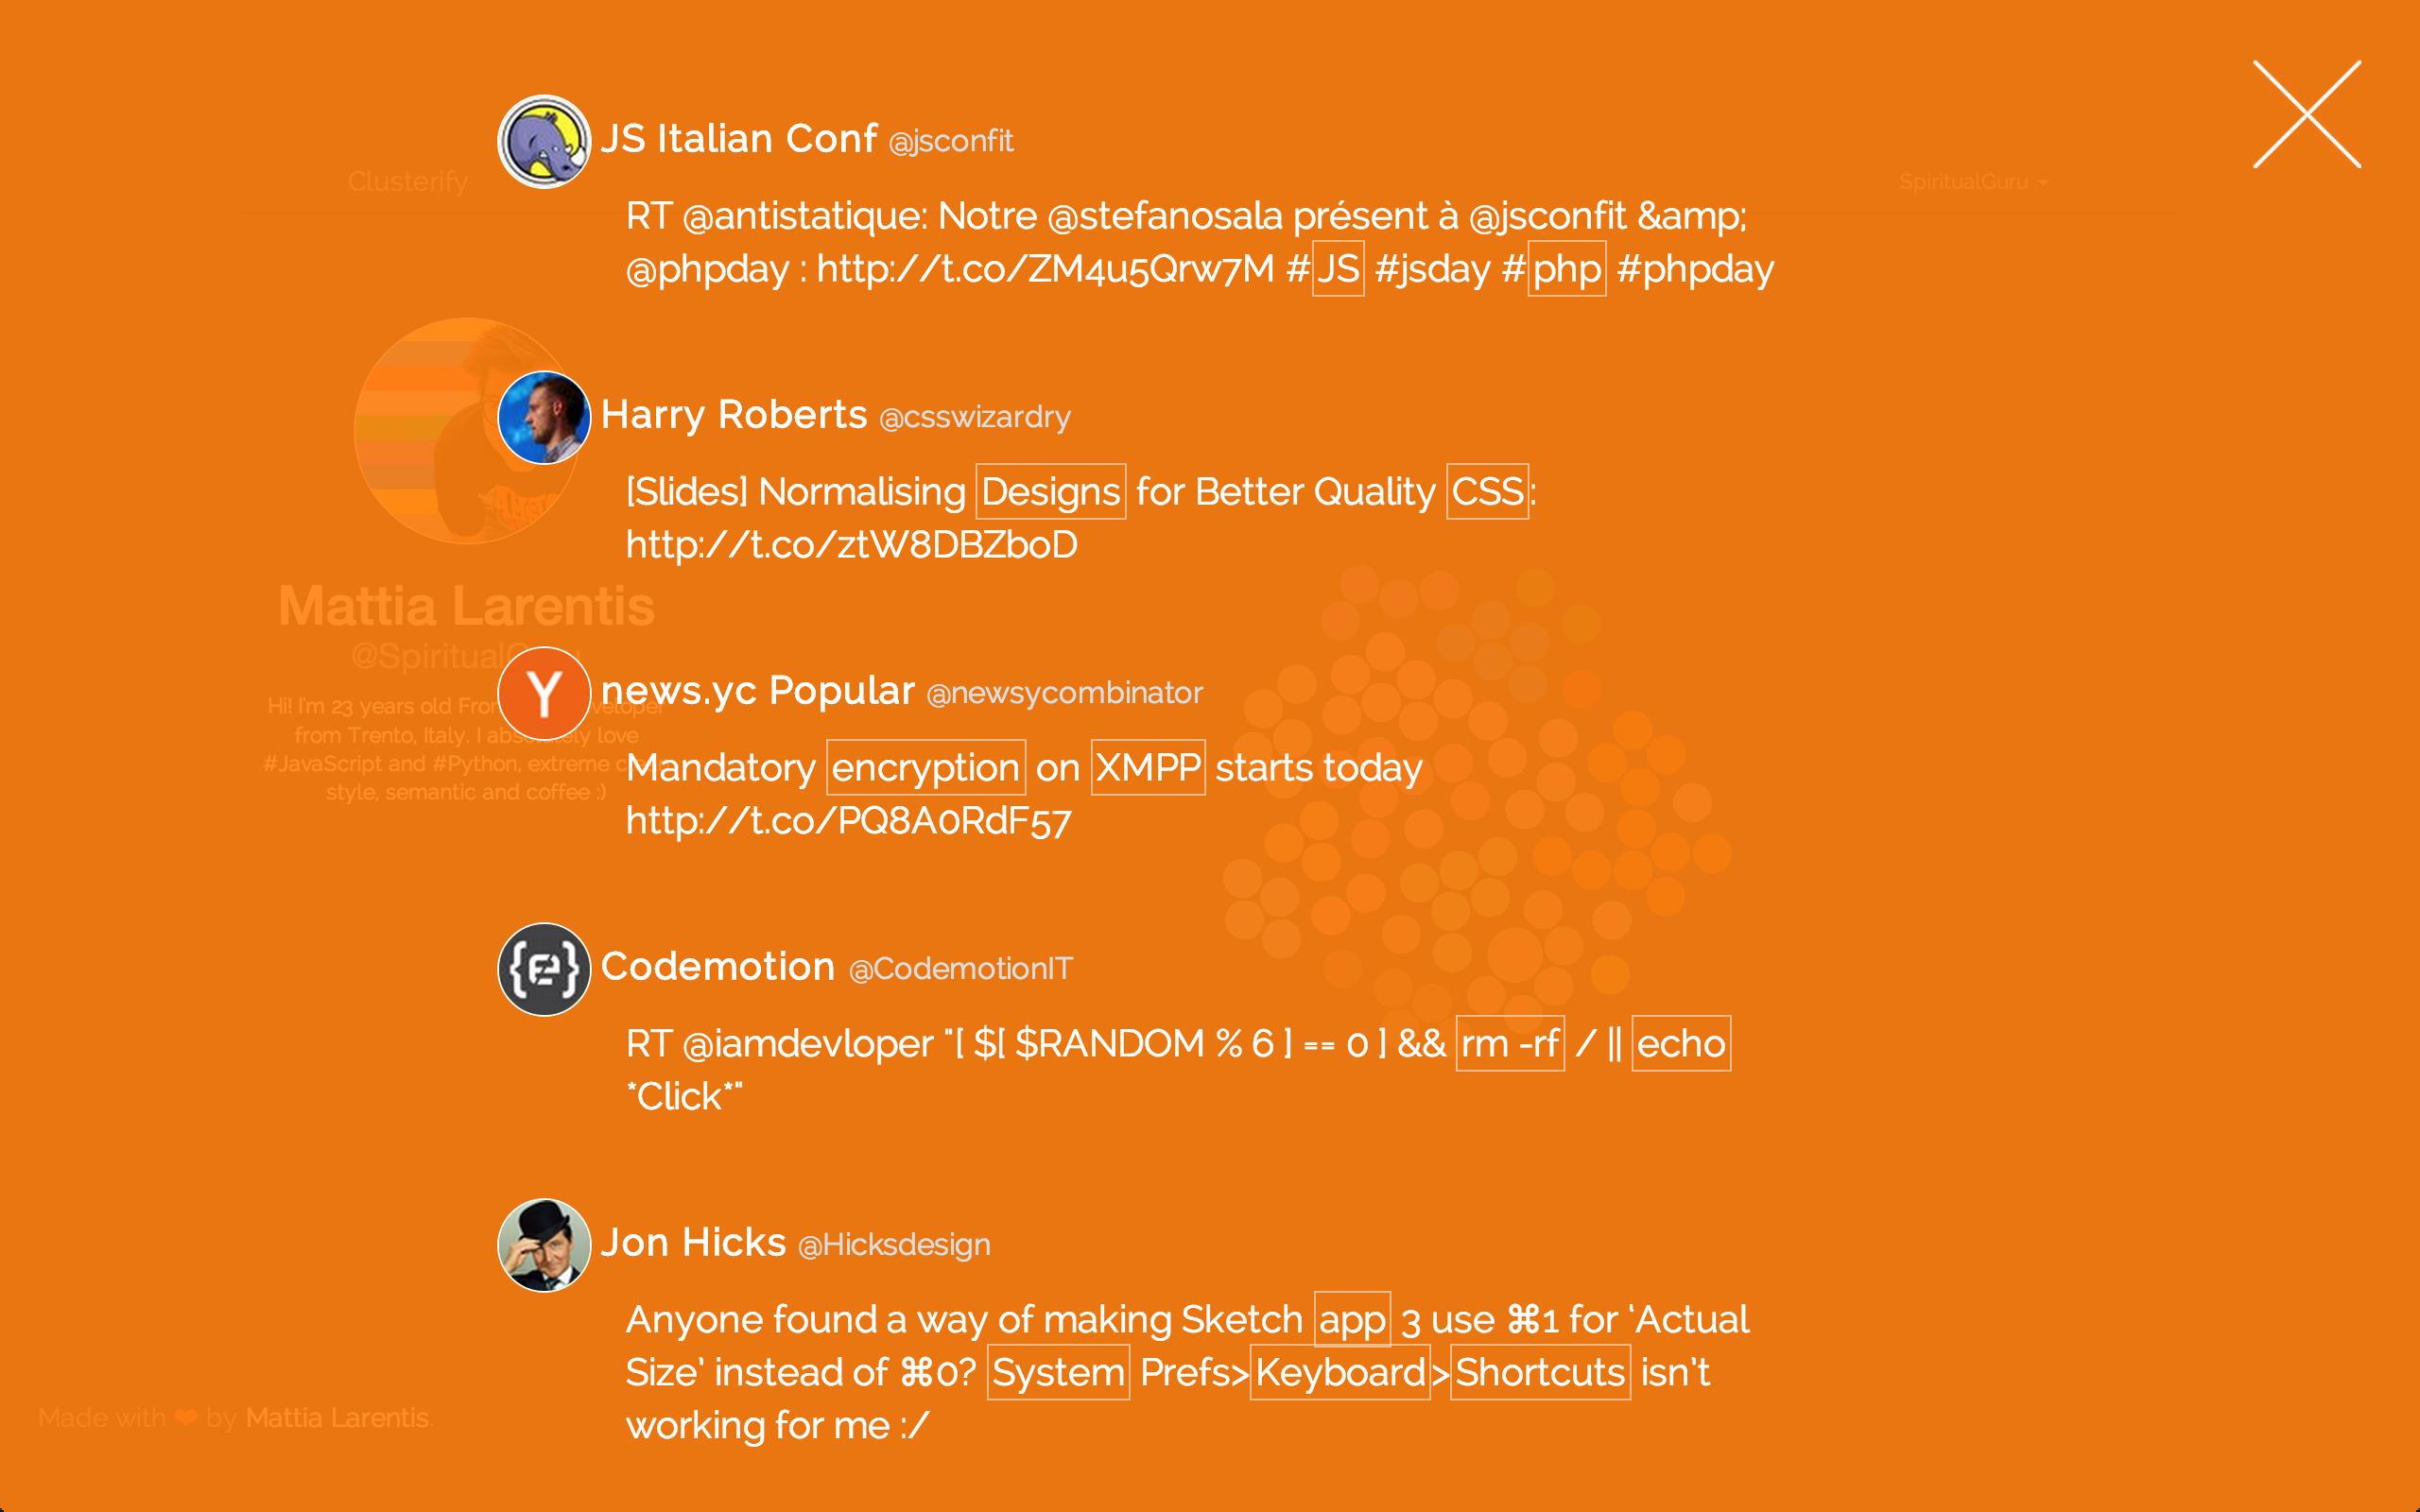
\includegraphics[width=\textwidth]{img/clusterify/tweet.png}
        	\end{figure}
        
        	\begin{figure}[p]
		\textbf{Storico delle elaborazioni}: pagina dove sono visibili tutte le elaborazioni che un utente ha lanciato.\\

        		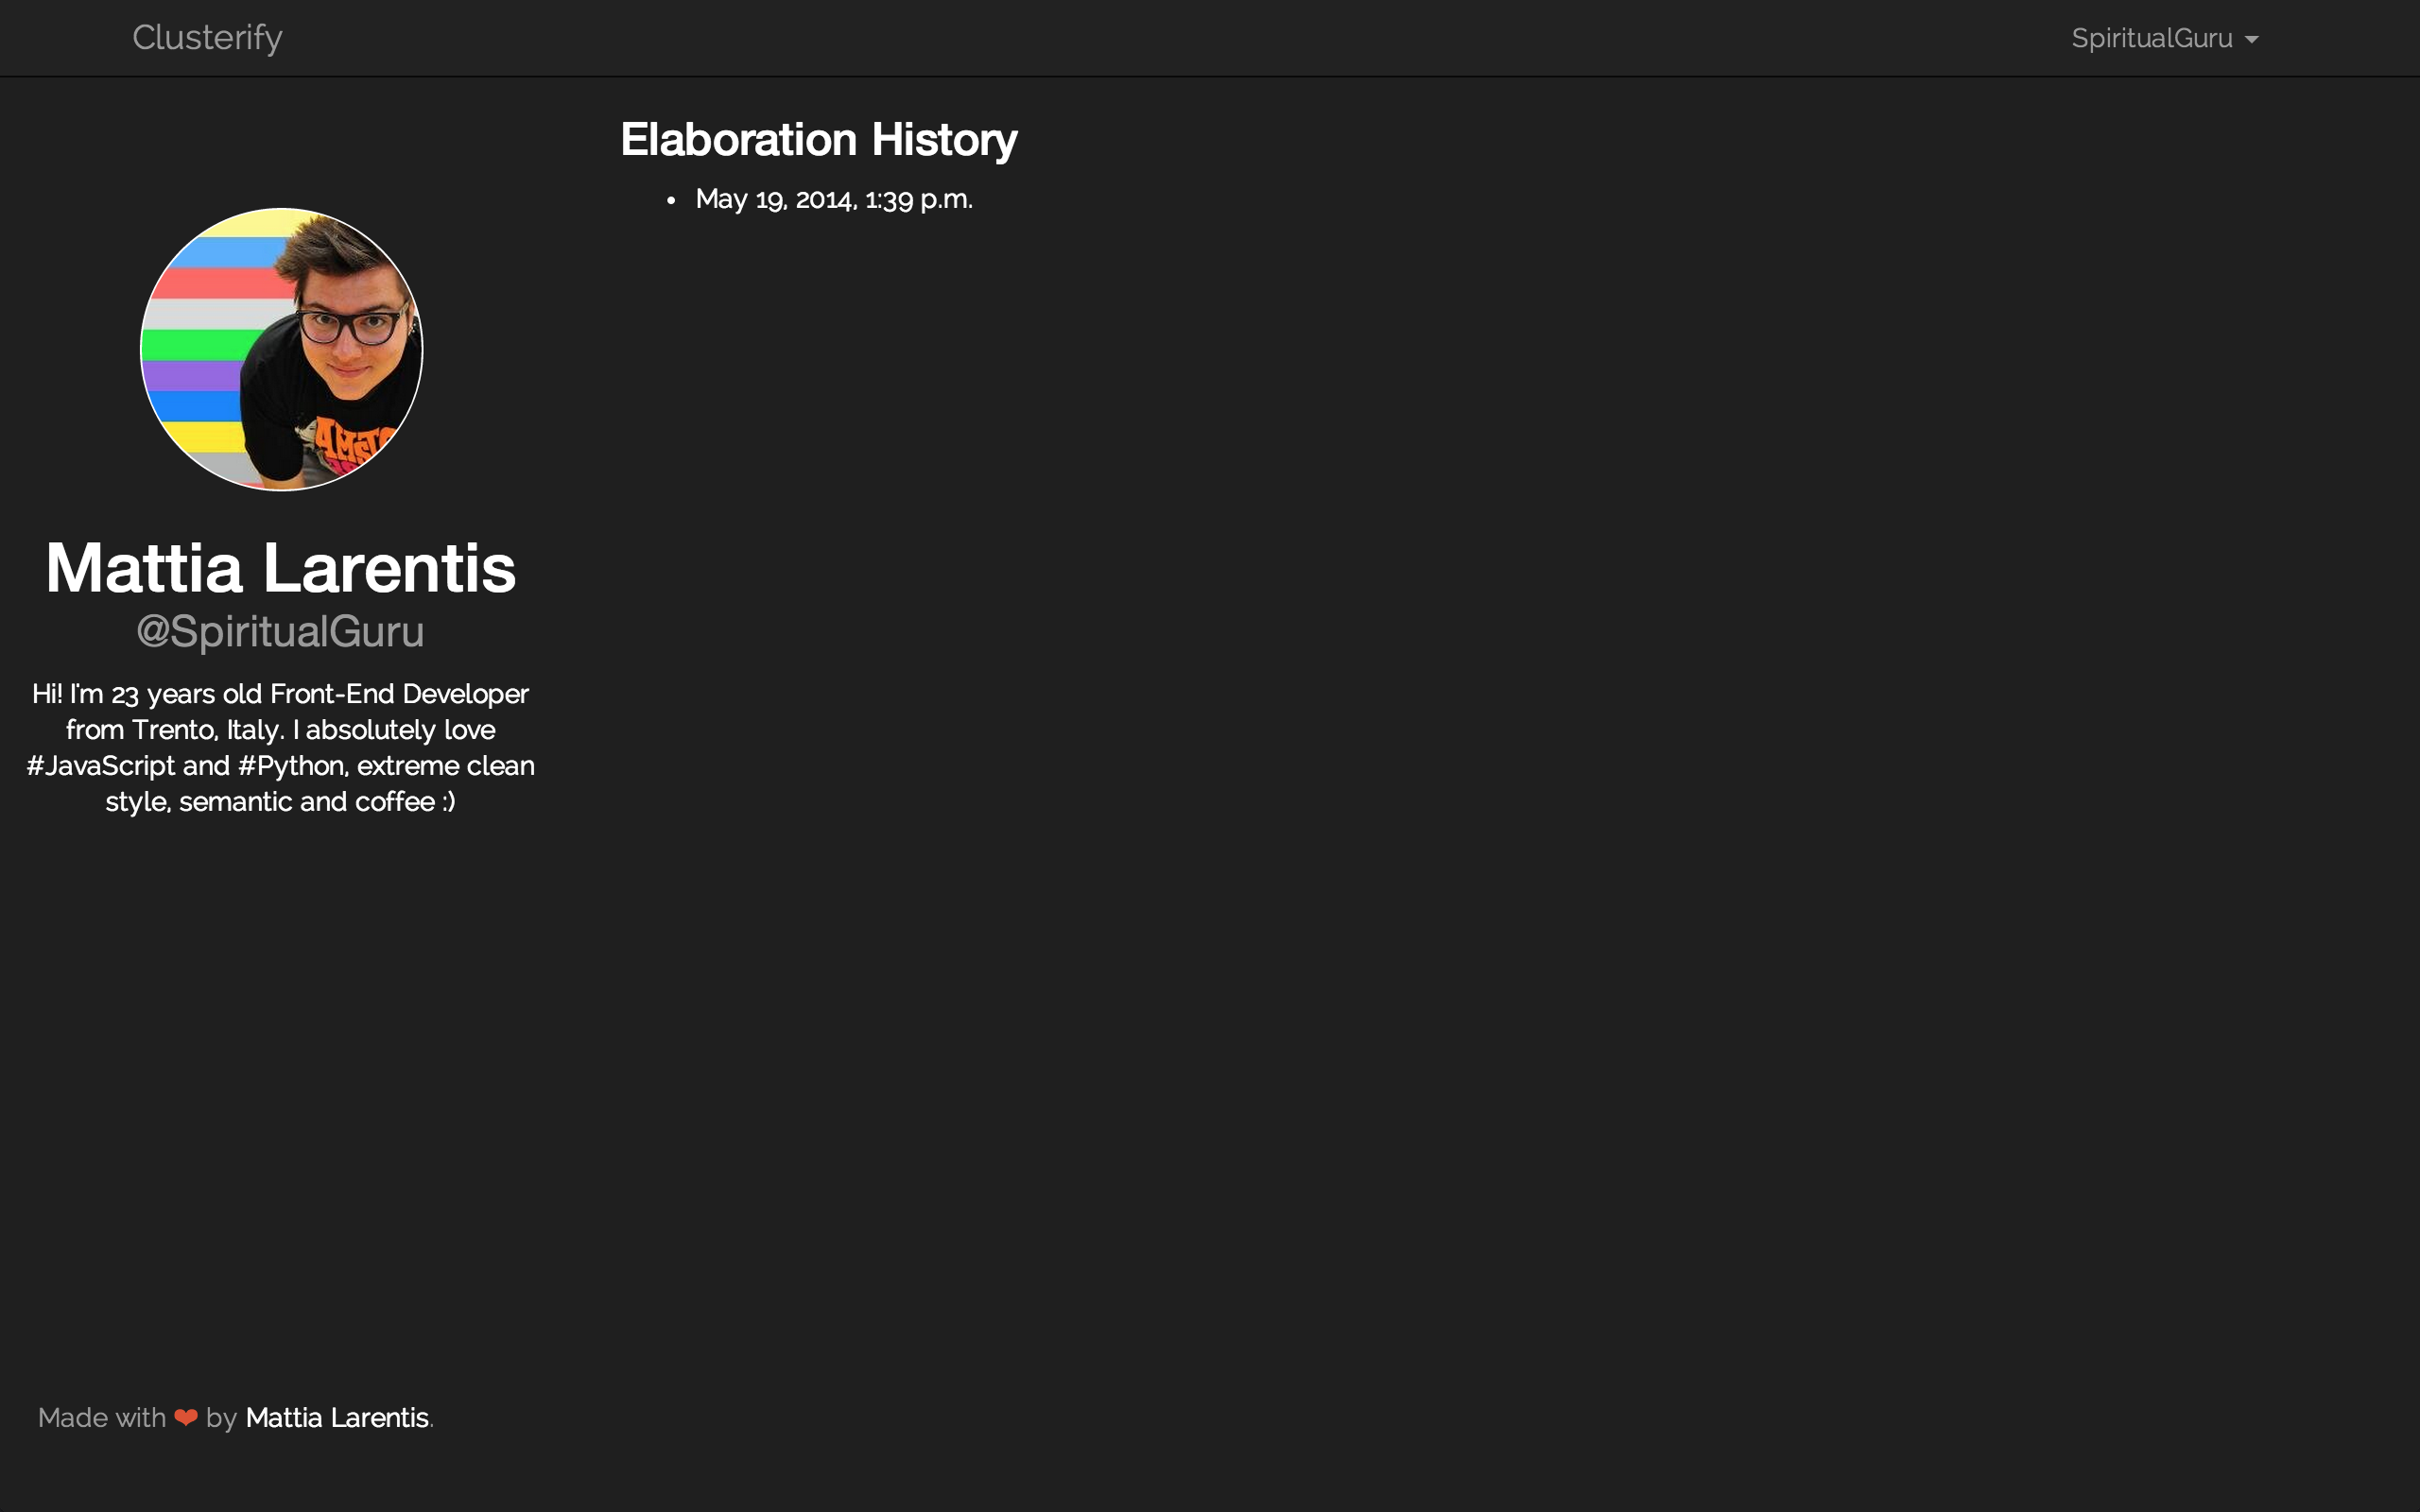
\includegraphics[width=\textwidth]{img/clusterify/history.png}
        	\end{figure}            
	
	\newpage
	Successivamente, si è proposta la soluzione a 10 utenti, gli stessi che hanno valutato l'algoritmo di clustering, per capire se fossero sorti altri problemi nell'implementazione della piattaforma. 

	Tutti gli utenti sono rimasti soddisfatti ed il 60\% ha detto che lo userebbe nella vita reale.


